\chapter{\label{ch:4-madc_model_application}MDC Model Application and BVL adaptation}

In this chapter, we will explore the application of the \textit{Multilevel Dynamic Conservation} (MDC) Model as a Documentation Model for digital archives. Therefore, we will define a descriptive metadata structure for creative works and apply it through two very different development platforms – Neo4j and GitHub repositories – as well as a file management system, Finder. These systems represent distinct application scenarios, which is why they were selected. Neo4j is a graph database management system (GDBMS) that is particularly powerful in applications involving complex relationships between data\footnote{Some of the most famous application to use Neo4j are Linkedin, Netflix, PayPal, eBay, Uber, etc.}. GitHub is a collaborative version control platform for developers, allowing the creation, storage, management, and sharing of code and multimedia files. Finder is the Macintosh operating system's file manager and graphical user interface for organising folders and files and launching applications. The descriptive metadata schemes used in the three applications are adopted from existing descriptive and metadata systems, more or less specific to artworks and creative works. The organisation and structure of these metadata schemas will differ slightly across the three application systems, as each has its own development and application tools.\\
We wanted to apply the MDC model to these very different systems to highlight its abstraction and independence from any specific development platform while showcasing its adaptability. As emphasised in the previous chapter, this is the main strength of the model and the reason why we have called it a meta-model: it describes how a conservation model should be modelled and thus can be applied to different scenarios, with different levels of complexity and definition, without requiring specialised application skills. The application of the MDC model on these systems is illustrated by the case studies presented in Appendices~\ref{ax:a-michele_sambin_videoloop}, \ref{ax:b-hybrid_reactivation_il_caos_delle_sfere}, \ref{ax:c-the_score_in_live_electronics_music}, and \ref{ax:d-sustainability_and_longevity_of_nimes}. Appendices~\ref{ax:a-michele_sambin_videoloop} and \ref{ax:b-hybrid_reactivation_il_caos_delle_sfere} describe two complex artworks archived through Neo4j. Appendix~\ref{ax:d-sustainability_and_longevity_of_nimes} discusses two case studies related to research projects in the NIME field, archived and documented through a GitHub repository. Finally, Appendix~\ref{ax:c-the_score_in_live_electronics_music} focuses on the reactivation and study of scores from live electronic music works, which were stored using Finder for organising personal documentation and files (``actor archive''). We will refer to these case studies when presenting the various systems and their use according to the MDC model. Please refer to the respective chapters for more details about the case studies.\\
At the end of this chapter, we will also cover the adaptation of \textit{Baalman Visual Language} (BVL) used for the Modular Instruction Framework (MIF). In addition to the book Composing Interaction (Baalman, 2023), there is a repository where the BVL's author provides materials for using the language\footnote{\url{https://github.com/composing-interactions/ci-visual-language?tab=readme-ov-file} (last access 15/11/201)}. The repository includes SVG and PNG files with various blocks, arrows, and fonts. In the case studies discussed, we chose not to use the provided files as we found them somewhat tricky and especially limiting. Therefore, we decided to move away from the original graphical aspect of the language but extracted its key concepts (level division, differentiations and connections between blocks, etc.). The graphic reconstruction of the model was done using Diagrams.net, a cross-platform, online graph drawing software for creating diagrams such as flowcharts, wireframes, network diagrams, and more. In this case, we applied Baalman’s logic and concepts independently of the graphical language in a different environment.\\
The language was also applied to the case studies, and we will provide some examples from the studies in this context.\\
This chapter does not discuss the application of the CATTA reactivation workflow. Indeed, the reactivation process is explained for each case study, following the various steps during reactivation. Therefore, to see the application of the CATTA reactivation workflow, please refer to Appendices~\ref{ax:a-michele_sambin_videoloop}, \ref{ax:b-hybrid_reactivation_il_caos_delle_sfere}, ~\ref{ax:c-the_score_in_live_electronics_music}, and \ref{ax:d-sustainability_and_longevity_of_nimes}.

\section{Descriptive metadata schema and structure}
Before discussing the application of the MDC model through the different systems, it is essential to introduce the metadata schemas used to describe the various archived items and their relation and organisation. In this application, we did not introduce novel metadata schemas but instead adopted existing ones for the different types of descriptions needed for archiving. In this case, we used descriptive metadata schemas that were useful for describing the artworks and research projects covered in the case studies, which included different types of items. These include sensors, computers, smartphones, audio and video equipment, software, musical instruments, self-made boxes as well as artworks, the people and organisation involved, the iterations of the works, and more. Each of these elements requires specific and different fields of description.\\
Below, we list the main descriptive metadata schemas used in the archive and their application in the context of the MDC model.

\subsection{Artwork and iterations}
Although partially, the description of the creative work, which corresponds to the first macro level of the MDC model, can relate to the \textit{Identity Reports} developed and used by museums. Here, we consider six \textit{Identity Reports}: the one developed by the \textit{Media Conservation Initiative} (MCI) project at MoMA\footnote{MoMa’s Media Conservation Initiative (MCI)'s \textit{Identity Report} \url{https://static1.squarespace.com/static/5835fd7c15d5db57b19535bd/t/5c0042351ae6cf02642c2674/1543520821538/_Identity_Report_Template.pdf} (last accessed, 17/11/2024).}; the one developed by the \textit{Media Preservation Initiative} (MPI) project at the Whitney Museum of American Art\footnote{Whitney Museum of American Art’s Media Preservation Initiative (MPI)'s \textit{Identity report} \url{https://whitneymedia.org/assets/generic_file/1655/MPI_Identity_Report_Template.pdf} (last accessed, 17/11/2024).}; the one developed by the \textit{Time-based Media \& Digital Art Working Group} at the Smithsonian American Art Museum (SAAM)\footnote{ The SAAM’s Time-based Media \& Digital Art Working Group's \textit{Identity report} \url{https://whitneymedia.org/assets/generic_file/1655/MPI_Identity_Report_Template.pdf} (last accessed, 17/11/2024).}; the one developed by the Guggenheim\footnote{Guggenheim’s \textit{Identity Report} \url{https://www.guggenheim.org/wp-content/uploads/2019/12/guggenheim-identity-report-cant-help-myself-sun-yuan-peng-yu.pdf} (last accessed, 17/11/2024).}; the \textit{Cataloguing Form} developed by the DOCAM Research Alliance\footnote{The DOCAM cataloguing form \url{https://www.docam.ca/en/tools/cataloguing-form.html} (last accessed, 17/11/2024).}; and the \textit{Installation Specification} developed by the \textit{Matters in Media Art} project\footnote{The Matters in Media Art's Installation Specificiation can be found at the following link: \url{https://mattersinmediaart.org/acquiring-time-based-media-art.html} (last accessed, 17/11/2024).}
.\\
All the \textit{Identity Reports} share many common sections, as we have already seen in Cahpter~\ref{ch:1-state_of_the_art} when referring to the Guggenheim \textit{Identity Report}. Here, we can summarise these sections as follows: 1) \textit{Identification} (Artwork identification), 2) \textit{Description} (identity of the artwork), 3) \textit{History of Exhibitions and Iterations}, 4) \textit{Anatomy of the Artwork}, 5) \textit{Risk and Resources}, 6) \textit{Installation Parameters}, and 7) \textit{Technical Requirements and Parameters}. It is clear that when using the MDC model, the various fields of the \textit{Identity Report} are distributed across the different sub-levels of the archive. The \textit{History of Exhibitions and Iterations} and all description fields are used at the individual \textit{Iteration File} (IF) level. \textit{Anatomy of the Artwork}, \textit{Installation Parameters}, and \textit{Technical Requirements and Parameters} are described at the \textit{bit} and \textit{data} levels. Only \textit{Identification}, \textit{Description}, and \textit{Risk and Resources} are used at the artwork level. Therefore, the artwork can be defined using with the fields in Table~\ref{tab:c4-artwork}.

\begin{longtable}{|p{0.35\textwidth}|p{0.15\textwidth}|p{0.4\textwidth}|}
    \caption{Artwork Metadata Schema} \label{tab:c4-artwork} \\
    \hline
    \textbf{Field} & \textbf{Value} & \textbf{Description} \\
    \hline
    \endfirsthead

    \scriptsize id                      & \scriptsize String                                            &  \scriptsize Item Identifier. \\
    \hline
    \scriptsize id:title                   & \scriptsize String                                            &  \scriptsize Title of the creative work.\\
    \hline
    \scriptsize id:dateCreated             & \scriptsize Date                                              &  \scriptsize The date of the creative work creation is in the format ISO8601 (e.g., yyyy-mm-dd).\\
    \hline
    \scriptsize id:artist                  & \scriptsize \textcolor{uniudColor3}{Person}[]                 &  \scriptsize The person(s) who created the creative work. \\
    \hline
    \scriptsize id:picture                 & \scriptsize \textcolor{uniudColor3}{Image}                    &  \scriptsize Link to a single image (\textit{experience} item) that represents the creative work. \\
    \hline
    \scriptsize id:description             & \scriptsize String                                            &  \scriptsize Description of the creative work. \\
    \hline
    \scriptsize id:conservationStatement   & \scriptsize String                                            &  \scriptsize A conservation statement with the essential aspects to consider in order to conserve the artwork.\\
    \hline
    \scriptsize id:iterationSeries         & \scriptsize \textcolor{uniudColor3}{Iteration}[]              &  \scriptsize A series of iterations (manifestations) of the creative work. \\
    \hline
    \scriptsize id:bibliographySeries      & \scriptsize \textcolor{uniudColor3}{Book}[] \textcolor{uniudColor3}{Paper}[] ...   &  \scriptsize A series of reference texts. \\
    \hline

\end{longtable}
Here, we decided to identify the artwork with the most general aspects, reducing the number of description fields. For example, the description of the artwork is usually divided into several sections, which cover the curatorial and artistic aspects, technical details, statements from the artists and collaborators, and so on. Here, we simplify this into a single \textit{description} field. The same applies to the \textit{conservationStatement} field. Additionally, we do not use the common field for \textit{medium} or \textit{medium lines}, which are typically used in \textit{identification}. The medium can be derived from the \textit{bit}s and \textit{data} for each \textit{Iteration File}.\\
The process for the \textit{Iteration Report} is very similar. Here, we focused on the \textit{Iteration Reports} from the Guggenheim\footnote{ Guggenheim’s \textit{Iteration Report} \url{https://www.guggenheim.org/wp-content/uploads/2015/11/guggenheim-conservation-iteration-report-2012.pdf} (last accessed, 18/11/2024).} and the \textit{Time-based Media \& Digital Art Working Group} at the Smithsonian American Art Museum (SAAM) \footnote{SAAM’s \textit{Iteration Report} \url{https://www.si.edu/tbma/resource/iteration-report} (last accessed, 18/11/2024).}– which are very similar – the \textit{Exhibition Report} from the \textit{Media Preservation Initiative} (MPI) project at the Whitney Museum of American Art\footnote{Whitney Msueum of American Art’s \textit{Exhibition Report} \url{https://whitneymedia.org/assets/generic_file/1657/MPI_Exhibition_Report_Template.pdf} (last accessed, 18/11/2024).}, and the \textit{Documentation for Technological Changes} from the DOCAM research alliance\footnote{DOCAM’s \textit{Documentation for technological changes} \url{https://www.docam.ca/en/tools/documentation-for-technological-changes.html} (last accessed, 18/11/2024).}. Therefore, each iteration is described with the fields in Table~\ref{tab:c4-iteration}.

\begin{longtable}{|p{0.35\textwidth}|p{0.15\textwidth}|p{0.4\textwidth}|}
    \caption{Iteration Metadata Schema} \label{tab:c4-iteration} \\
    \hline
    \textbf{Field} & \textbf{Value} & \textbf{Description} \\
    \hline
    \endfirsthead
    \scriptsize id                      & \scriptsize String                                            &  \scriptsize Item Identifier. \\
    \hline
    \scriptsize it:title                   & \scriptsize String, \textcolor{uniudColor3}{Event}            &  \scriptsize Event or Iteration/Exhibition title.\\
    \hline
    \scriptsize it:date                    & \scriptsize Date                                              &  \scriptsize The exhibition date in the format ISO8601 (e.g., yyyy-mm-dd). For describing the exhibition period: [startDate, endDate].\\
    \hline
    \scriptsize it:venue                   & \scriptsize \textcolor{uniudColor3}{Place}                    &  \scriptsize The Place in which the iteration took place. \\
    \hline
    \scriptsize it:curator, performer, mediaTechnichian, ...                 & \scriptsize \textcolor{uniudColor3}{Person}[]                    &  \scriptsize All the people involved in the iteration with their role\footnote{Based on the \textit{Iteration reports} studied we can have: \textit{Curator}(s), \textit{Exhibition Designer}(s), \textit{Media Technician}(s), \textit{Conservator}(s), \textit{Registrar}(s), \textit{Artist}(s), \textit{Artist Assistant}(s), \textit{Fabricator}(s), \textit{Art Handler}(s), \textit{Consultant}(s), \textit{External Company}, \textit{and Other}(s). The \textit{Iteration Reports} usually consider only exhibition such as installation and they do not include performers, that we would like to add in the description of the iteration since would be helpful to describe our case studies.}..\\
    \hline
    \scriptsize it:description             & \scriptsize String                                            &  \scriptsize Description of the iteration. \\
    \hline
    \scriptsize it:picture                 & \scriptsize \textcolor{uniudColor3}{Image}                    &  \scriptsize Link to a single \textit{experience} item that represents the iteration of the artwork.\\
    \hline
    \scriptsize it:note                    & \scriptsize String                                            &  \scriptsize Note about the iteration that can comprehend problems related to the installation and rehearsal, technological changes, and other essential details. \\
    \hline
    \scriptsize it:bit                     & \scriptsize \textcolor{uniudColor3}{AudioEquip}[], \textcolor{uniudColor3}{VideoEquip}[], ...   &  \scriptsize List of \textit{bit} items related to the iteration.\\
    \hline
   \scriptsize  it:data                    & \scriptsize \textcolor{uniudColor3}{Image}[], \textcolor{uniudColor3}{Doc}[], ...   &  \scriptsize List of \textit{data} items related to the iteration.\\
    \hline
    \scriptsize it:experience              & \scriptsize \textcolor{uniudColor3}{Image}[], \textcolor{uniudColor3}{Video}[], \textcolor{uniudColor3}{Paper}[], ...   &  \scriptsize List of \textit{experience} items related to the iteration.\\
    \hline
\end{longtable}

In this case, the description fields have also been significantly reduced compared to the \textit{Iteration Reports} we studied. Once again, much of the information from these reports is spread across the various upper and lower levels of the MDC model and can be easily derived by looking at the archive as a whole (as we will see in the following subsections).\\
Schema value types such as \textit{Person}, \textit{Image}, \textit{Video}, \textit{Iteration}, \textit{Book}, \textit{Paper} and so on (highlighted in blue in the tables) refer to other metadata schemas. For example, \textit{iterationSeries} in the \textit{Creative Work} metadata schema refers to multiple Iteration metadata schemas (multiple as indicated by the two square brackets).

\subsection{Person, organisation, place, and event}
We use the metadata schemas defined by \textit{Schema.org} as a model to describe entities related to the artworks and their iterations—such as person, organisation, event, and place. \textit{Schema.org} is a community-driven initiative focused on creating, maintaining, and promoting schemas for structured data across the Internet, including web pages, email messages, and more.\\
According to \textit{Schema.org}, we define in Table~\ref{tab:c4-person}, with some necessary adjustments for the description area, the \textit{Person} metadata schema.

\begin{longtable}{|p{0.35\textwidth}|p{0.15\textwidth}|p{0.4\textwidth}|}
    \caption{Person Metadata Schema} \label{tab:c4-person} \\
    \hline
    \textbf{Field} & \textbf{Value} & \textbf{Description} \\
    \hline

    \scriptsize id                      & \scriptsize String                                            &  \scriptsize Item Identifier. \\
    \hline
    \scriptsize pe:givenName               & \scriptsize String                                             &  \scriptsize The first name of a Person.\\
    \hline
    \scriptsize pe:familyName              & \scriptsize String                                             &  \scriptsize The last name of a Person.\\
    \hline
    \scriptsize pe:birthDate               & \scriptsize Date                                             &  \scriptsize Date of birth in the ISO8601 format.\\
    \hline
    \scriptsize pe:birthPlace              & \scriptsize \textcolor{uniudColor3}{Place}                    &  \scriptsize The place where the person was born.\\
    \hline
    \scriptsize pe:deathDate               & \scriptsize Date                                             &  \scriptsize Date of death in the ISO8601 format.\\
    \hline
    \scriptsize pe:deathPlace              & \scriptsize \textcolor{uniudColor3}{Place}                    &  \scriptsize The place where the person died.\\
    \hline
    \scriptsize pe:nationality             & \scriptsize String                                       &  \scriptsize Nationality of the person.\\
    \hline
    \scriptsize pe:biography               & \scriptsize String                                       &  \scriptsize A biography of the person.\\
    \hline
    \scriptsize pe:website                 & \scriptsize URL                                       &  \scriptsize Website of the person.\\
    \hline

\end{longtable}

Table~\ref{tab:c4-organisation} show the \textit{Organisation} metadata schema according to \textit{Scema.org}. In this context, the organization should be viewed as a group of people structured in either a private or institutional manner.

\begin{longtable}{|p{0.35\textwidth}|p{0.15\textwidth}|p{0.4\textwidth}|}
    \caption{Organisation Metadata Schema} \label{tab:c4-organisation} \\
    \hline
    \textbf{Field} & \textbf{Value} & \textbf{Description} \\
    \hline

    \scriptsize id                      & \scriptsize String                                            &  \scriptsize Item Identifier. \\
    \hline
    \scriptsize or:legalName             & \scriptsize String                                            &  \scriptsize The official name of the organisation. \\
    \hline
    \scriptsize or:address               & \scriptsize \textcolor{uniudColor3}{Place}[], Address         &  \scriptsize The organisation's physical address according to the Universal Postal Union (UDU) recommendation. \\
    \hline
    \scriptsize or:member                & \scriptsize \textcolor{uniudColor3}{Person}[], \textcolor{uniudColor3}{Organisation}[] &  \scriptsize Person(s) or Organisation(s) members of the organisation. \\
    \hline
    \scriptsize or:description           & \scriptsize Text                                             &  \scriptsize Description of the organisation. \\
    \hline
    \scriptsize or:website                 & \scriptsize URL                                              & \scriptsize  Website of the organisation. \\
    \hline

\end{longtable}

Table~\ref{tab:c4-place} show the \textit{Place} metadata schema according to \textit{Scema.org}. 

\begin{longtable}{|p{0.35\textwidth}|p{0.15\textwidth}|p{0.4\textwidth}|}
    \caption{Place Metadata Schema} \label{tab:c4-place} \\
    \hline
    \textbf{Field} & \textbf{Value} & \textbf{Description} \\
    \hline

    \scriptsize id                      & \scriptsize String                                            &  \scriptsize Item Identifier. \\
    \hline
    \scriptsize pl:legalName             & \scriptsize String                                            &  \scriptsize The official name of the place. \\
    \hline
    \scriptsize pl:address               & \scriptsize Address                                          &  \scriptsize The place's physical address according to the Universal Postal Union (UDU) recommendation. \\
    \hline
    \scriptsize pl:description           & \scriptsize Text                                             &  \scriptsize Description of the place. \\
    \hline
    \scriptsize pl:website                 & \scriptsize URL                                              &  \scriptsize Website of the place. \\
    \hline

\end{longtable}

The last metadata schema referred to \textit{Schema.org} is the \textit{Event} metadata schema in Table~\ref{tab:c4-event}.

\begin{longtable}{|p{0.35\textwidth}|p{0.15\textwidth}|p{0.4\textwidth}|}
    \caption{Event Metadata Schema} \label{tab:c4-event} \\
    \hline
    \textbf{Field} & \textbf{Value} & \textbf{Description} \\
    \hline

    \scriptsize id                      & \scriptsize String                                            &  \scriptsize Item Identifier. \\
    \hline
    \scriptsize ev:name                  & \scriptsize String                                            &  \scriptsize Name of the event. \\
    \hline
    \scriptsize ev:startDate             & \scriptsize Date                                              &  \scriptsize Beginning of the event in the ISO8601 format. \\
    \hline
    \scriptsize ev:endDate               & \scriptsize Date                                              &  \scriptsize End of the event in the ISO8601 format. \\
    \hline
    \scriptsize ev:location              & \scriptsize \textcolor{uniudColor3}{Place}                    &  \scriptsize The place in which the event took place. \\
    \hline
    \scriptsize ev:organiser             & \scriptsize \textcolor{uniudColor3}{Person[]}, \textcolor{uniudColor3}{Organisation[]}   &  \scriptsize Organiser(s) of the event. \\
    \hline
    \scriptsize ev:description           & \scriptsize String                                            &  \scriptsize Description of the event. \\
    \hline
    \scriptsize ev:website                 & \scriptsize URL                                              & \scriptsize  Website of the event. \\
    \hline

\end{longtable}

For each type of metadata schema, we selected the essential fields (which can be extended by referring to the original metadata schema\footnote{\textit{Person} Metadata schema \url{https://schema.org/Person} (last accessed 17/11/2024); \textit{Organisation} Metadata schema \url{https://schema.org/Organization} (last accessed 17/11/2024); \textit{Place} metadata schema \url{https://schema.org/Place} (last accessed 17/11/2024); \textit{Event} metadata schema \url{https://schema.org/Event} (last accessed 17/11/2024).}). We added specific fields, such as \textit{biography} in the \textit{Person} schema (where the original \textit{description} field could be used) and \textit{website} for all.

\subsection{Audio and video equipments}
There are no specific standards for describing audio physical devices, such as audio mixers, sound cards, microphones, etc. However, we can combine the general description from \textit{Dublin Core} with the technical specifications from the Audio Engineering Society's AES57 standard \cite{AES57}.\\
The description of an audio mixer could follow these fields in Table~\ref{tab:c4-mixer}.

\begin{longtable}{|p{0.35\textwidth}|p{0.15\textwidth}|p{0.4\textwidth}|}
    \caption{Mixer Metadata Schema} \label{tab:c4-mixer} \\
    \hline
    \textbf{Field} & \textbf{Value} & \textbf{Description} \\
    \hline

    \scriptsize id                      & \scriptsize String           & \scriptsize Item Identifier. \\
    \hline
    \scriptsize db:title                & \scriptsize String           & \scriptsize The name and model of the mixer. \\
    \hline
    \scriptsize db:description          & \scriptsize String           & \scriptsize A brief summary of the mixer's features and specifications. \\
    \hline
    \scriptsize db:subject              & \scriptsize String           & \scriptsize A brief description of the mixer's primary purpose or application. \\
    \hline
    \scriptsize db:dateCreated          & \scriptsize Date             & \scriptsize The creation date of the equipment in ISO8601 format. \\
    \hline
    \scriptsize db:creator              & \scriptsize \textcolor{uniudColor3}{Person}[], \textcolor{uniudColor3}{Organisation}[], String & \scriptsize Person(s) or organization(s) that created the mixer. \\
    \hline
    \scriptsize db:publisher            & \scriptsize \textcolor{uniudColor3}{Person}[], \textcolor{uniudColor3}{Organisation}[], String & \scriptsize Publisher or manufacturer of the mixer. \\
    \hline
    \scriptsize db:format               & \scriptsize String           & \scriptsize Specifies the format or category of the mixer (e.g., Analog Mixing Console). \\
    \hline
    \scriptsize db:relation             & \scriptsize String           & \scriptsize Identifies the series or family to which the mixer belongs. \\
    \hline
    \scriptsize eas57:analogInterfaces  & \scriptsize String           & \scriptsize Specifies the analog input/output interfaces available on the device. \\
    \hline
    \scriptsize eas57:audioDataEncoding & \scriptsize String           & \scriptsize Indicates the type of audio data encoding, such as analog or digital. \\
    \hline
    \scriptsize eas57:dynamicRange      & \scriptsize String           & \scriptsize The dynamic range of the equipment, typically measured in dB. \\
    \hline
    \scriptsize eas57:numberOfChannels  & \scriptsize Integer          & \scriptsize The number of channels the equipment can handle. \\
    \hline
    \scriptsize eas57:powerRequirements & \scriptsize String           & \scriptsize Details about the equipment's power source or requirements. \\
    \hline
    \scriptsize eas57:signalToNoiseRatio& \scriptsize String           & \scriptsize The signal-to-noise ratio, typically measured in dB, indicating audio clarity. \\
    \hline
    \scriptsize eas57:dimensions        & \scriptsize String           & \scriptsize The physical dimensions of the equipment in width x height x depth format. \\
    \hline
    \scriptsize eas57:weight            & \scriptsize String           & \scriptsize The weight of the equipment, typically measured in kilograms. \\
    \hline

\end{longtable}

Similarly, no specific standards exist for describing video physical devices—such as LCD screens, cameras, etc. Again, we use \textit{Dublin Core} for general descriptive metadata, combined with the technical standards from the Society of Motion Picture and Television Engineers \cite{SMPTE}, which capture technical specifications.\\
The description of a generic LCD monitor could follow the fields listed in Table~\ref{tab:c4-video}.

\begin{longtable}{|p{0.35\textwidth}|p{0.15\textwidth}|p{0.4\textwidth}|}
    \caption{Monitor Metadata Schema} \label{tab:c4-monitor} \\
    \hline
    \textbf{Field} & \textbf{Value} & \textbf{Description} \\
    \hline

    \scriptsize id                      & \scriptsize String           & \scriptsize Item Identifier. \\
    \hline
    dc:title                & \scriptsize String           & \scriptsize The name and model of the monitor. \\
    \hline
    \scriptsize dc:description          & \scriptsize String           & \scriptsize A brief summary of the monitor's features and specifications. \\
    \hline
    \scriptsize dc:subject              & \scriptsize String           & \scriptsize A brief description of the monitor's primary purpose or classification. \\
    \hline
    \scriptsize dc:dateCreated          & \scriptsize Date             & \scriptsize The release or creation date of the monitor in ISO8601 format. \\
    \hline
    \scriptsize dc:creator              & \scriptsize \scriptsize \textcolor{uniudColor3}{Person}[], \textcolor{uniudColor3}{Organisation}[], String           & \scriptsize Person(s) or Organization(s) that created the monitor. \\
    \hline
    \scriptsize dc:publisher            & \scriptsize \scriptsize \textcolor{uniudColor3}{Person}[], \textcolor{uniudColor3}{Organisation}[], String           & \scriptsize Person(s) or Organization(s) responsible for producing the monitor. \\
    \hline
    \scriptsize dc:format               & \scriptsize String           & \scriptsize The format and specifications of the monitor, such as resolution and technology. \\
    \hline
    \scriptsize dc:relation             & \scriptsize String           & \scriptsize The series or family to which the monitor belongs. \\
    \hline
    \scriptsize smpte:aspectRatio      & \scriptsize String           & \scriptsize The ratio of the width to the height of the display. \\
    \hline
    \scriptsize smpte:brightness        & \scriptsize String           & \scriptsize The brightness of the display, typically measured in cd/m². \\
    \hline
    \scriptsize smpte:colorSpace       & \scriptsize String           & \scriptsize The color space supported by the display, such as sRGB. \\
    \hline
    \scriptsize smpte:contrastRatio    & \scriptsize String           & \scriptsize The contrast ratio, which measures the difference between the darkest and brightest output. \\
    \hline
    \scriptsize smpte:contributor       & \scriptsize String           & \scriptsize The individual or team that contributed to the product development. \\
    \hline
    \scriptsize smpte:coverage          & \scriptsize String           & \scriptsize The geographical coverage or availability of the product. \\
    \hline
    \scriptsize smpte:frameRate        & \scriptsize String           & \scriptsize The maximum refresh rate of the display, measured in Hz. \\
    \hline
    \scriptsize smpte:interface         & \scriptsize String           & \scriptsize The input/output interfaces supported by the monitor, such as HDMI or VGA. \\
    \hline
    \scriptsize smpte:powerConsumption & \scriptsize String           & \scriptsize The amount of power the monitor consumes, typically measured in watts. \\
    \hline
    \scriptsize smpte:resolution        & \scriptsize String           & \scriptsize The resolution of the display in pixels, such as 1920x1080. \\
    \hline
    \scriptsize smpte:syncSupport      & \scriptsize String           & \scriptsize The synchronization technology supported by the monitor, such as FreeSync. \\
    \hline

\end{longtable}


\subsection{Computer hardware and software}
To describe desktop computers, laptops, single-board computers, microcontrollers, and commercial application software, we can use the \textit{Common Information Model} (CIM) standard developed by the Distributed Management Task Force (DMTF) \cite{CIM}. The CIM standard provides a framework for describing the management of information technology (IT) infrastructure, including hardware, software, and network resources. This system is powerful because it allows for a clear separation of various computer components, such as processors, RAM, storage, etc., and also helps establish relationships with software components.\\
An example of a computer system described using the CIM metadata schema is in table~\ref{tab:c4-computer}

\begin{longtable}{|p{0.45\textwidth}|p{0.15\textwidth}|p{0.3\textwidth}|}
    \caption{Computer System Metadata Schema} \label{tab:c4-computer} \\
    \hline
    \textbf{Field} & \textbf{Value} & \textbf{Description} \\
    \hline

    \scriptsize id                                    & \scriptsize String                         & \scriptsize Item Identifier. \\
    \hline
    \scriptsize cim:ComputerSystem.elementName        & \scriptsize String                         & \scriptsize The name of the laptop computer system. \\
    \hline
    \scriptsize cim:ComputerSystem.Name               & \scriptsize String                         & \scriptsize The model name of the laptop. \\
    \hline
    \scriptsize cim:ComputerSystem.Manufacturer       & \scriptsize String, \textcolor{uniudColor3}{Organisation}[], \textcolor{uniudColor3}{Person}[]     & \scriptsize The manufacturer of the laptop. \\
    \hline
    \scriptsize cim:ComputerSystem.Model              & \scriptsize String                         & \scriptsize The model number or specific name of the laptop. \\
    \hline
    \scriptsize cim:ComputerSystem.OperatingSystem    & \scriptsize \textcolor{uniudColor3}{cim:OperatingSystem}[]          & \scriptsize The operating system installed on the laptop. \\
    \hline
    \scriptsize cim:ComputerSystem.Processor          & \scriptsize \textcolor{uniudColor3}{cim:Processor}[]                & \scriptsize The processor(s) installed on the laptop. \\
    \hline
    \scriptsize cim:ComputerSystem.Memory             & \scriptsize \textcolor{uniudColor3}{cim:Memory}[]                   & \scriptsize The memory(s) installed on the laptop. \\
    \hline
    \scriptsize cim:ComputerSystem:StorageVolume      & \scriptsize \textcolor{uniudColor3}{cim:StorageVolume}[]            & \scriptsize The storage volume(s) installed on the laptop. \\
    \hline
    \scriptsize cim:ComputerSystem:Display            & \scriptsize \textcolor{uniudColor3}{smpte:Display}                  & \scriptsize The display of the laptop. \\
    \hline
    \scriptsize …                                     & \scriptsize …                              & \scriptsize … \\
    \hline

\end{longtable}

In this case, the values \textit{cim:OperatingSystem}, \textit{cim:Processor}, \textit{cim:Memory}, \textit{cim:StorageVolume} and many others refer to relations to other CIM metadata schemas. The \textit{smpte:Display} can be related to the \textit{Monitor} Metadata Schema, and the same thing could be done for a sound card and other Audio or Video Equipments.
An example of a metadata schema for the \textit{operating system} is in table~\ref{tab:c4-os}

\begin{longtable}{|p{0.45\textwidth}|p{0.15\textwidth}|p{0.3\textwidth}|}
    \caption{Operating System Metadata Schema} \label{tab:c4-os} \\
    \hline
    \textbf{Field} & \textbf{Value} & \textbf{Description} \\
    \hline

    \scriptsize id                                    & \scriptsize String                         & \scriptsize Item Identifier. \\
    \hline
    \scriptsize cim:OperatingSystem.elementName       & \scriptsize String                         & \scriptsize The name of the Operating system. \\
    \hline
    \scriptsize cim:ComputerSystem.Name               & \scriptsize String                         & \scriptsize The model name of the operating system. \\
    \hline
    \scriptsize cim:OperatingSystem.Manufacturer      & \scriptsize String, \textcolor{uniudColor3}{Organisation}, \textcolor{uniudColor3}{Person}     & \scriptsize The manufacturer of the Operating System. \\
    \hline
    \scriptsize cim:OperatingSystem.OSArchitecture    & \scriptsize String                         & \scriptsize The operating system's architecture (e.g., x64, x86, ARM). \\
    \hline
    \scriptsize cim:OperatingSystem.OSType            & \scriptsize String                         & \scriptsize The operating system type (e.g., Desktop, Server, Embedded). \\
    \hline
    \scriptsize cim:OperatingSystem.Platform          & \scriptsize String                         & \scriptsize The platform that the operating system is designed to run on (e.g., Windows). \\
    \hline
    \scriptsize …                                     & \scriptsize …                              & \scriptsize … \\
    \hline

\end{longtable}

For software applications, we can also use the CIM standard, as shown in table~\ref{tab:c4-software}:

\begin{longtable}{|p{0.45\textwidth}|p{0.15\textwidth}|p{0.3\textwidth}|}
    \caption{Software Application Metadata Schema} \label{tab:c4-software} \\
    \hline
    \textbf{Field} & \textbf{Value} & \textbf{Description} \\
    \hline

    \scriptsize id                                    & \scriptsize String                         & \scriptsize Item Identifier. \\
    \hline
    \scriptsize cim:SoftwareElement.ElementName       & \scriptsize String                         & \scriptsize The name of the software application. \\
    \hline
    \scriptsize cim:SoftwareElement.Name              & \scriptsize String                         & \scriptsize The full name and version of the software application. \\
    \hline
    \scriptsize cim:SoftwareElement.Manufacturer      & \scriptsize String, \textcolor{uniudColor3}{Organisation}, \textcolor{uniudColor3}{Person}     & \scriptsize The manufacturer of the software application. \\
    \hline
    \scriptsize cim:SoftwareElement.Version           & \scriptsize String                         & \scriptsize The version number of the software. \\
    \hline
    \scriptsize cim:SoftwareElement.OperatingSystem   & \scriptsize \textcolor{uniudColor3}{cim:OperatingSystem}[]          & \scriptsize The operating systems supported by the software. \\
    \hline
    \scriptsize cim:SoftwareElement.Description       & \scriptsize String                         & \scriptsize A brief description of the software’s purpose and functionality. \\
    \hline
    …                                     & \scriptsize …                              & … \\
    \hline

\end{longtable}

For non-commercial, original software, we have chosen to use \textit{CodeMeta}, a metadata schema developed for scientific research. It is designed to facilitate the sharing and reusing code and software\footnote{Codemeta project website \url{https://codemeta.github.io/} (last accessed 19/11/2024).}. An example is given in table~\ref{tab:c4-original-software} \footnote{To generate a metadata schema with the \textit{CodeMeta Generator v3.0} at the link \url{https://codemeta.github.io/codemeta-generator/} (last accessed 19/11/2024).}
.

\begin{longtable}{|p{0.45\textwidth}|p{0.15\textwidth}|p{0.3\textwidth}|}
    \caption{Original Software Metadata Schema} \label{tab:c4-original-software} \\
    \hline
    \textbf{Field} & \textbf{Value} & \textbf{Description} \\
    \hline

    \scriptsize id                                    & \scriptsize String                         & \scriptsize Item Identifier. \\
    \hline
    \scriptsize cm:Name                               & \scriptsize String                         & \scriptsize The name of the original software. \\
    \hline
    \scriptsize cm:Description                        & \scriptsize String                         & \scriptsize Description of the software. \\
    \hline
    \scriptsize cm:CreationDate                       & \scriptsize Date                           & \scriptsize Date of the software creation according to the ISO8601 format. \\
    \hline
   \scriptsize  cm:FirstReleaseDate                   & \scriptsize Date                           & \scriptsize Date of the first software release according to the ISO8601 format. \\
    \hline
    \scriptsize cm:License                            & \scriptsize URL[]                          & \scriptsize Attributed licence(s). \\
    \hline
    \scriptsize cm:UniqueIdentifier                   & \scriptsize String                         & \scriptsize An identifier for the software. \\
    \hline
    \scriptsize cm:Author                             & \scriptsize String, \textcolor{uniudColor3}{Person}[], \textcolor{uniudColor3}{Organisation}[]        & \scriptsize Person(s) or Organisation(s) that created the software. \\
    \hline
    \scriptsize cm:Keywords                           & \scriptsize String                         & \scriptsize Relevant keywords that describe the software. \\
    \hline
    \scriptsize cm:ProgrammingLanguage                & \scriptsize String, \textcolor{uniudColor3}{cim:SoftwareApplication} & \scriptsize The programming language with which the software has been developed (e.g. Java, Python, etc.). \\
    \hline
    \scriptsize cm:RuntimePlatform                    & \scriptsize String, \textcolor{uniudColor3}{cim:SoftwareApplication} & \scriptsize Runtime application for running the software (.NET, JVM, etc.). \\
    \hline
    \scriptsize cm:OperatingSystem                    & \scriptsize \textcolor{uniudColor3}{cim:OperatingSystem}            & \scriptsize Operating system for running the software. \\
    \hline
    \scriptsize cm:OtherSoftwareRequirement           & \scriptsize String, \textcolor{uniudColor3}{cim:SoftwareApplication}, URL & \scriptsize Other requirements include libraries, multimedia files, etc. \\
    \hline
    \scriptsize cm:VersionNumber                      & \scriptsize String                         & \scriptsize The current version of the software. \\
    \hline
    \scriptsize …                                     & \scriptsize …                              & \scriptsize … \\
    \hline

\end{longtable}

\subsection{Sensors}
\textit{Sensor Model Language} (SensorML) is a specific description system for various types of sensors \cite{SensorML}. It provides a structured and semantically linked way to define processes and components involved in measuring and transforming observations. SensorML also provides metadata schemas for sensors, actuators, and computational processes applied before and after measurements. Using this system, we can describe not only sensors but also potentiometers and other components typically used in creating original devices for artworks.\\
A metadata schema for a temperature sensor could follow the fields listed in table~\ref{tab:c4-sensor}:


\begin{longtable}{|p{0.35\textwidth}|p{0.15\textwidth}|p{0.4\textwidth}|}
    \caption{Sensor (Temperature Sensor) Metadata Schema} \label{tab:c4-temperature-sensor} \\
    \hline
    \textbf{Field} & \textbf{Value} & \textbf{Description} \\
    \hline

    \scriptsize …id                                    & \scriptsize String                         & \scriptsize …Item Identifier. \\
    \hline
    \scriptsize …sml:Sensor.Name                       & \scriptsize String                         & \scriptsize …The name or model of the temperature sensor. \\
    \hline
    \scriptsize …sml:Sensor.Description                & \scriptsize String                         & \scriptsize …A short description of the sensor’s functionality. \\
    \hline
    \scriptsize …sml:Sensor.Manufacturer               & \scriptsize String, \textcolor{uniudColor3}{Organisation}, \textcolor{uniudColor3}{Person}     & \scriptsize …The manufacturer of the temperature sensor. \\
    \hline
    \scriptsize …sml:Sensor.Model                      & \scriptsize String                         & \scriptsize …The specific model of the temperature sensor. \\
    \hline
    \scriptsize …sml:Sensor.Type                       & \scriptsize String                         & \scriptsize …The type of measurement the sensor is designed for (in this case, temperature). \\
    \hline
    \scriptsize …sml:Sensor.MeasurementUnit            & \scriptsize String                         & \scriptsize …The unit of measurement used by the sensor (e.g., Celsius, Fahrenheit). \\
    \hline
    \scriptsize …sml:Sensor.OperatingRange             & \scriptsize String                         & \scriptsize …The sensor's operational range indicates the minimum and maximum temperature it can measure. \\
    \hline
    \scriptsize …sml:Sensor.Sensitivity                & \scriptsize String                         & \scriptsize …The temperature sensor's sensitivity represents the smallest detectable change in temperature. \\
    \hline
    \scriptsize …sml:Sensor.Accuracy                   & \scriptsize String                         & \scriptsize …The accuracy of the temperature measurements provided by the sensor. \\
    \hline
    \scriptsize ……                                     & \scriptsize …                              & \scriptsize …… \\
    \hline

\end{longtable}

\subsection{Multimedia files}
Many metadata schema standards exist for multimedia files, such as audio and video. In this case, we have adopted the multimedia content description standard from the Moving Picture Experts Group, MPEG-7 \cite{MPEG7}. Although it is used in a basic way here, this standard allows for a general description of the multimedia file and enables the storage of metadata related to a timecode, thus keeping track of events within the video.\\
An example of a video described using the MPEG-7 metadata schema is in table~\ref{tab:c4-video}:

\begin{longtable}{|p{0.35\textwidth}|p{0.15\textwidth}|p{0.4\textwidth}|}
    \caption{Video Metadata Schema} \label{tab:c4-video} \\
    \hline
    \textbf{Field} & \textbf{Value} & \textbf{Description} \\
    \hline

    \scriptsize id                                    & \scriptsize String                         & \scriptsize Item Identifier. \\
    \hline
    \scriptsize mpeg7:VideoFile.Title                 & \scriptsize String                         & \scriptsize The title of the video file. \\
    \hline
    \scriptsize mpeg7:VideoFile.Creator               & \scriptsize String, \textcolor{uniudColor3}{Person}[], \textcolor{uniudColor3}{Organisation}[]        & \scriptsize The creators of the video (e.g., director, producer). \\
    \hline
    \scriptsize mpeg7:VideoFile.Description           & \scriptsize String                         & \scriptsize A brief description or summary of the video content. \\
    \hline
    \scriptsize mpeg7:VideoFile.Format                & \scriptsize String                         & \scriptsize The video file format (e.g., MP4, AVI, MKV). \\
    \hline
    \scriptsize mpeg7:VideoFile.Duration              & \scriptsize String                         & \scriptsize The duration of the video file. \\
    \hline
    \scriptsize mpeg7:VideoFile.FrameRate             & \scriptsize String                         & \scriptsize The frame rate of the video (e.g., 30 frames per second). \\
    \hline
    \scriptsize mpeg7:VideoFile.AspectRatio           & \scriptsize String                         & \scriptsize The aspect ratio of the video (e.g., 16:9, 4:3). \\
    \hline
    \scriptsize mpeg7:VideoFile.Bitrate               & \scriptsize String                         & \scriptsize The bitrate of the video (e.g., 5 Mbps). \\
    \hline
    \scriptsize mpeg7:VideoFile.Codec                 & \scriptsize String                         & \scriptsize The video codec used (e.g., H.264, VP9). \\
    \hline
    \scriptsize mpeg7:VideoFile.AudioFeatures         & \scriptsize Map                            & \scriptsize Audio features of the video file, including language and audio type (e.g., stereo, mono). E.g. {"Language": "English", "AudioType": "Stereo"} \\
    \hline
    \scriptsize mpeg7:VideoFile.VisualFeatures        & \scriptsize Map                            & \scriptsize Visual features of the video file, such as dominant colours and scene changes. E.g. {"ColorDominance": "Green", "SceneChange": "4"} \\
    \hline
    \scriptsize mpeg7:VideoFile.Chapters              & \scriptsize Map[]                          & \scriptsize Video chapter information, including start and end time and title. E.g. [{"start": "00:00:00", "end": "00:30:00", "title": "Introduction to Wildlife"}] \\
    \hline
    …                                     & \scriptsize …                              & … \\
    \hline

\end{longtable}

\subsection{Other and generic}
In order to describe many other different items, we have chosen to use \textit{Dublin Core}, a general standard description metadata schema \cite{DublinCore}. We primarily use this system to describe musical instruments and digital images and to define data items (usually stored as flowchart images and diagrams).\\
A concrete example of describing the Disklavier piano used in the case study \textit{Il Caos delle sfere} (in Appendix~\ref{ax:b-hybrid_reactivation_il_caos_delle_sfere}) is given in table~\ref{tab:c4-disklavier}

\begin{longtable}{|p{0.35 \textwidth}|p{0.55\textwidth}|}
    \caption{Yamaha Disklavier Metadata Schema} \label{tab:c4-yamaha-disklavier} \\
    \hline
    \textbf{Field} & \textbf{Value} \\
    \hline

    \scriptsize id                                    & \scriptsize 4d30-a5be-5fbdedd27bc2:28 \\
    \hline
    \scriptsize dc:title                              & \scriptsize Yamaha Disklavier Model D1 \\
    \hline
    \scriptsize dc:creator                            & \scriptsize Yamaha Corporation \\
    \hline
    \scriptsize dc:subject                            & \scriptsize Player Piano, Digital Piano, MIDI \\
    \hline
    \scriptsize dc:description                        & \scriptsize The Yamaha Disklavier is a player piano that combines the tradition of acoustic pianos with modern digital features, allowing for MIDI-controlled performance and music playback. \\
    \hline
    \scriptsize dc:publisher                          & \scriptsize Yamaha Corporation \\
    \hline
    \scriptsize dc:contributor                        & \scriptsize Various artists, composers \\
    \hline
    \scriptsize dc:date                               & \scriptsize 2023-11-18 \\
    \hline
    \scriptsize dc:type                               & \scriptsize Musical Instrument \\
    \hline
    \scriptsize dc:format                             & \scriptsize Acoustic and Digital (MIDI-capable) \\
    \hline
    \scriptsize dc:relation                           & \scriptsize MIDI, Music Software, Digital Music Files \\
    \hline
    \scriptsize dc:coverage                           & \scriptsize Global (Available in major music stores worldwide) \\
    \hline
    \scriptsize dc:identifier                         & \scriptsize \url{https://europe.yamaha.com/en/products/musical_instruments/pianos/disklavier/index.html} \\
    \hline

\end{longtable}


We use the \textit{BibTeX} system to describe resources and references such as books, articles, interviews, websites, etc., mainly in conjunction with \LaTeX\space documents. This system is both a tool and a format for describing and managing lists of references.\\
We can describe a generic book with the field in table~\ref{tab:c4-book}.

\begin{longtable}{|p{0.35\textwidth}|p{0.15\textwidth}|p{0.4\textwidth}|}
    \caption{Book Metadata Schema} \label{tab:c4-book} \\
    \hline
    \textbf{Field} & \textbf{Value} & \textbf{Description} \\
    \hline

    \scriptsize id                                    & \scriptsize String                         & \scriptsize Item Identifier. \\
    \hline
    \scriptsize bibtex:title                          & \scriptsize String                         & \scriptsize The title of the book. \\
    \hline
    \scriptsize bibtex:author                         & \scriptsize \textcolor{uniudColor3}{Person}[] & \scriptsize The author(s) of the book. \\
    \hline
    \scriptsize bibtex:publisher                      & \scriptsize String                         & \scriptsize The publisher of the book. \\
    \hline
    \scriptsize bibtex:year                           & \scriptsize Date                           & \scriptsize The year of the publication in the ISO8601 format. \\
    \hline
   \scriptsize  bibtex:volume                         & \scriptsize String                         & \scriptsize The volume of the book. \\
    \hline
    \scriptsize bibtex:address                        & \scriptsize String                         & \scriptsize The publisher's physical address according to the Universal Postal Union (UDU) recommendation. \\
    \hline
    \scriptsize bibtex:edition                        & \scriptsize String                         & \scriptsize The edition of the book. \\
    \hline
    \scriptsize bibtex:isbn                           & \scriptsize String                         & \scriptsize The International Standard Book Number (ISBN) of the book. \\
    \hline
    \scriptsize bibtex:url                            & \scriptsize String                         & \scriptsize A link related to the book. \\
    \hline

\end{longtable}

\subsection{General Metadata Structure}
Figure~\ref{fig:c4-metadata} shows the entire metadata structure we used for archiving according to the MDC model.


\begin{figure}[!h]
    \centering
    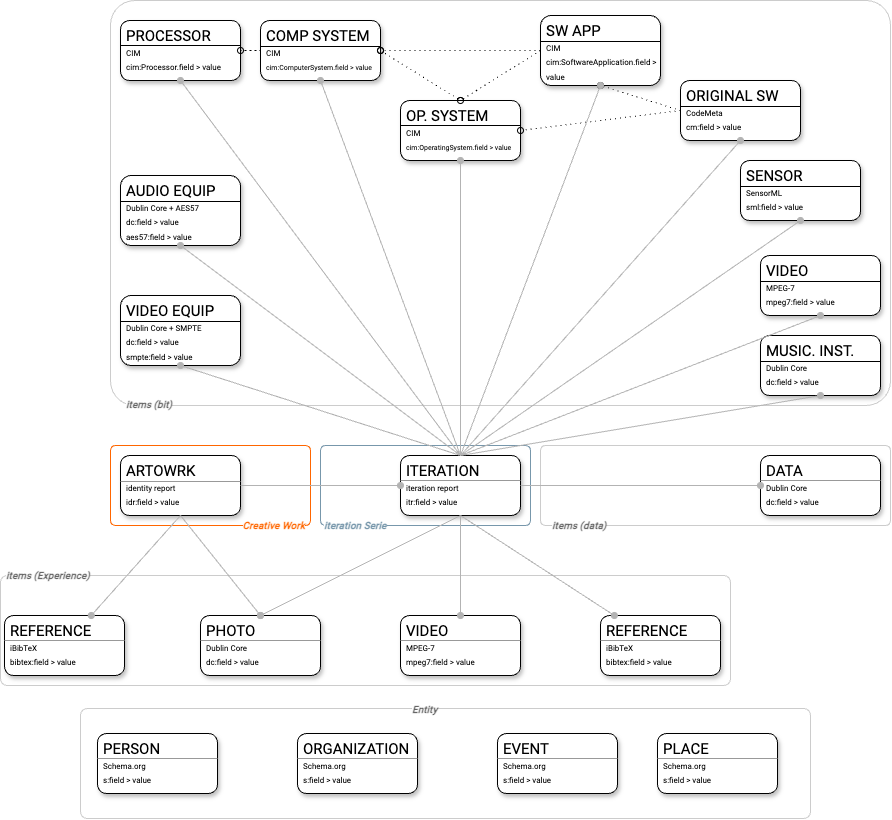
\includegraphics[width=\linewidth]{chapters/4-MDC_model_application/image/graph04-metadata.png}
    \caption{The metadata structure of our MDC Model application according to the metadata scehma introduced above.}
    \label{fig:c4-metadata}
\end{figure}

\section{MDC Model application}

\subsection{Neo4j Graph database application}

The application of the MDC model through the Neo4j graph database is by far the most complex, detailed, and complete case discussed in this text. This system was applied in case studies involving Michele Sambin’s \textit{videoloop} (Appendix~\ref{ax:a-michele_sambin_videoloop}) and Carlo De Pirro’s installation \textit{Il caos delle sfere} (Appendix~\ref{ax:b-hybrid_reactivation_il_caos_delle_sfere}). We will mainly focus on the case study of the \textit{videoloop}, as it presents a highly detailed case with intricate relationships between the various iterations of the artwork, as well as a large amount of documentation created before and during the reactivations.\\
As mentioned several times, Neo4j is a graph database and belongs to the NoSQL database family, which has gained popularity in the last decade as an alternative to traditional relational databases. It is especially useful for managing large volumes of interconnected data, enabling effective storage and retrieval \cite{lourencco2015choosing}. One of the main advantages of Graph databases is their efficiency in handling relationships between data, which were more challenging to manage in traditional relational databases. For this reason, graph databases are increasingly used in the context of social media.\\
Graph databases are easy to understand because their concept is based on graph theory, which is also one of the most useful structures for modelling objects and interactions. Graphs are mathematical structures used to model relationships between objects. In this context, graphs are defined by nodes (or vertices), edges (the relationships connecting the nodes), and properties representing information related to both the nodes and the edges \cite{guia2017graph}. In addition to being intuitive due to their natural representation of information (the graph), graph databases offer many other advantages that are highly relevant to our application context. First, they are much more flexible than relational databases, a characteristic common to all NoSQL databases. They are naturally additive, allowing us to add new types of data, such as nodes or relationships, easily without disrupting the overall structure and functionality of the application. The additive nature of graphs also means fewer migrations, which reduces maintenance overhead and risk.\\
Unlike relational databases and general NoSQL systems, graph databases store data as connected data, with nodes and edges at the same level. Relationships are ``first-class citizens'' of the graph data model, unlike other database management systems that require us to infer connections between entities using properties like foreign keys or out-of-band processing such as map-reduce. The connected data makes creating and querying relationships extremely agile and efficient, naturally enabling path formation. Moreover, relationships are not just links; they have direction and properties that straightforwardly allow us to define the semantic context of the paths. Therefore, graph databases are excellent for data mining operations \cite{robinson2013graph}.\\
Without considering all the computational performance advantages — also defined by the query languages implemented — compared to other types of databases \cite{vicknair2010comparison, guia2017graph, fernandes2018graph}, it is clear that graph databases can be highly efficient for both storing and retrieving information related to live media artworks. As discussed in Chapter~\ref{ch:1-state_of_the_art} and ~\ref{ch:2-new_conservation_paradigms}, one of the main features of live media art is its formal and material heterogeneity, as well as its relational heterogeneity with all the entities and elements it interacts with (the interdisciplinarity of the involved figures, the different types and spaces of exhibition, etc.). Representing this heterogeneity is undoubtedly enhanced by the flexibility offered by graph databases, where we can have a malleable data structure with the simplicity of adding new data structures for nodes and new types of relationships. Moreover, we must consider the complex relationships often found in live media art, including the intricate network of people involved in the artistic project, the exhibition, curation, and conservation of the works. The relationships intensify when we consider the components (\textit{bit}s) used in the works and all the documentation created, which, as seen in Chapter~\ref{ch:2-new_conservation_paradigms}, can trigger a complex network of relationships.\\
Additionally, there are relationships between the works and their iterations. In short, the relationships between elements of a live media artwork are one of the most important aspects in the context of their conservation. The MDC model is built upon this network of relationships, defining multidimensional connections between the artworks and their iterations, between iterations and components and documentation, between iterations and other iterations, and between all elements and the various entities involved (people, organisations, events, etc.). Therefore, the main strength of graph databases — their ability to enhance the relationship structure and derive semantic paths — is the key feature that led us to choose this database for archiving live media art.\\
Neo4j was chosen from many other graph database systems for its positive reviews and popularity. Over the years, this system has been tested and reviewed in both scientific and non-scientific contexts \cite{vicknair2010comparison, robinson2013graph, lourencco2015choosing, guia2017graph, fernandes2018graph, khan2023sql} and has consistently received positive feedback. Additionally, as seen on the DB-Engines website’s Graph DBMS Popularity Trend\footnote{DB-Engines Ranking of Graph DBMS \url{https://db-engines.com/en/ranking/graph+dbms} (last accessed, 19/12/2024)}, Neo4j is currently by far the most popular and fastest-growing graph database.\\
Neo4j is an open-source graph database implemented in Java, first released in 2007. It features its own query language, Cypher, developed by the database's creators, which allows users to manage all the information within the database. Cypher is relatively simple yet very powerful, enabling efficient and expressive query execution and updates to graph databases. Moreover, Neo4j offers an intuitive and user-friendly interface, allowing users to visualise the database as a graph or a JSON table, view all properties for each node and relationship, and quickly enter Cypher commands to work with and query the database.\\
In our application, we use Neo4j to collect all data related to the artworks and their documentation and, most importantly, to create all the relationships. We store all the files associated with artworks, such as source codes, videos, photos, instructions, scores, and so on, in a cloud system (Google Drive) and repositories (GitHub repository). The Neo4j database refers to each multimedia source through URLs.\\
In the following pages, we will explore Neo4j's use and potential in relation to the MDC model.\\
\newline
The first thing to mention is the creation of nodes and relationships. One main feature is that nodes and relationships can be labelled. The label is crucial because we use it to define the type of item and relationship. We could create a node with the label \texttt{CREATIVE\_WORK}, representing the artwork. This node can be easily created as follows:
\begin{lstlisting}[style=cypher]
CREATE (a:CREATIVE_WORK)
\end{lstlisting}
However, we need to assign all the properties of the artwork, which the metadata schema of the identity report will define.
\begin{lstlisting}[style=cypher]
CREATE (a:CREATIVE_WORK
{
       title: 'Il tempo consuma',
       dateCreated: date('1978'),
       description: '...',
       conservationStatement: '...'
}
)
\end{lstlisting}
In this way, we will create the node for the artwork \textit{Il tempo consuma} by Michele Sambin, as shown in Figure~\ref{fig:c4-neo4j-creativework}.
\begin{figure}[!h]
    \centering
    
\includegraphics[width=0.165\linewidth]{chapters/4-MDC_model_application/image/neo4j-singlenode.png}
    \caption{Michele Sambin's artwork \textit{Il tempo consuma} neo4j node.}
    \label{fig:c4-neo4j-creativework}
\end{figure}
However, if we refer to the \textit{Identity Report} metadata schema (Table~\ref{tab:c4-artwork}), we don’t see the \textit{artist}, \textit{photo}, \textit{iterationSeries}, and \textit{bibliographySeries} fields in this node\footnote{The \textit{id} field is automatically created by Neo4j when the node is created}. As we’ve seen in the metadata schema, these fields refer to other metadata schemas and, thus, other items. They can be added through relationships.\\
Assuming we’ve already added a \textit{Person} node for Michele Sambin, we can add the relationship artist with the following Cypher query:
\begin{lstlisting}[style=cypher]
MATCH (a:CREATIVE_WORK {title: 'Il tempo consuma'}), (p:PERSON {familyName: 'Sambin'})
CREATE (a)-[r:ARTIST]->(p)
\end{lstlisting}
In this case, we used the \texttt{MATCH} command to select the nodes representing \textit{Il tempo consuma} and \textit{Michele Sambin}. Then, we created a simple directional relationship from the artwork to the person, with \textit{artist} as a metadata field of the \textt{CREATIVE\_WORK} node. We can visualise this, as shown in Figure~\ref{fig:c4-neo4j-artworkrelation}.

\begin{figure}[!h]
    \centering
    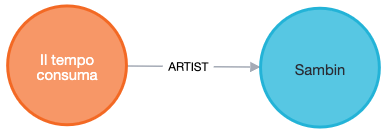
\includegraphics[width=0.5\linewidth]{chapters/4-MDC_model_application/image/neo4j-singlerelationship.png}
    \caption{The relationship between \texttt{CREATIVE\_WORK} and \texttt{PERSON} nodes through the \textit{artist} field of the \textit{Creative Work} metadata scehma.}
    \label{fig:c4-neo4j-artworkrelation}
\end{figure}

Figure~\ref{fig:c4-neo4j-artworkrelation} shows all the first-level relationships of the artwork Il tempo consuma, including the iterations, bibliography, and representative photo.
\begin{figure}[!h]
    \centering
    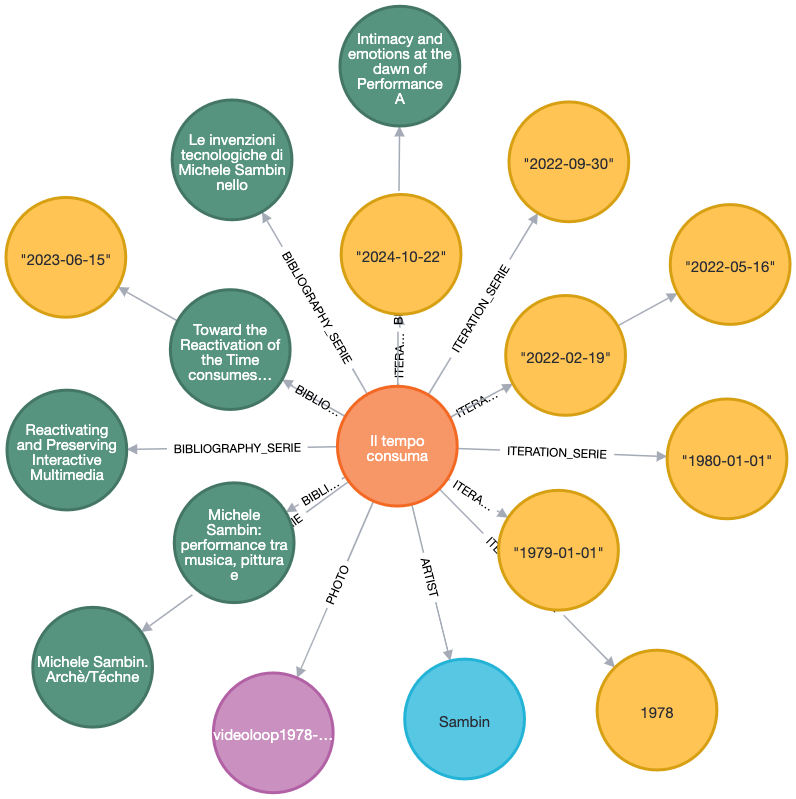
\includegraphics[width=1\linewidth]{chapters/4-MDC_model_application/image/neo4j-artworkrelation.png}
    \caption{First-level Neo4j relationships of \textit{Il tempo consuma} by Michele Sambin.}
    \label{fig:c4-neo4j-artworkrelation}
\end{figure}
One of the features of Neo4j that is very useful in our application context is that relationships can be more than just simple connections; they can also contain properties. With these properties, we can enhance the information about specific relationships. For example, the relationship \texttt{BIBLIOGRAPHY\_SERIE} between \textit{Il tempo consuma} and the monograph \textit{Michele Sambin: performance tra musica, pittura e video} \cite{lischi2014michele} can be expanded by specifying the pages where the authors discuss the \textit{videoloop} topic. The relationship would look like this (in JSON format):
\begin{lstlisting}[style=json]
{"start":0, "end":12, "type": 'BIBLIOGRAPHY_SERIE', "properties": {"pages": ['117-122', '252']}
\end{lstlisting}
So, the relationship between node 0 (\textit{Il tempo consuma}) and node 12 (the monograph)\footnote{Node numbering in Neo4j is based on the order in which nodes are created. Each node is assigned a unique identifier (ID) that reflects its creation sequence.} is of type \texttt{BIBLIOGRAPHY\_SERIE} and can be found in two sections, one on page 117 and the other on page 252.\\
Another very useful case for utilising this feature is the characterisation of performers. One of the iterations of the \textit{videoloop} reactivation was performed by multiple people, in addition to Michele Sambin and the author of this text (usually video and audio director), as is typical in the performance of the digitalised version of the \textit{videoloop}. In Figure~\ref{fig:c4-neo4j-performer}, we can see all the performers of the performance at the Sala dei Giganti in Padua on 16 May 2022, during the \textit{Opera Libera} event, part of the celebrations for the 800th anniversary of the University of Padua.
\begin{figure}[!h]
    \centering
    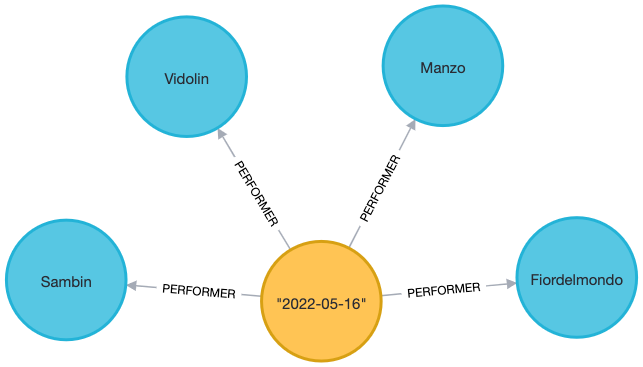
\includegraphics[width=0.75\linewidth]{chapters/4-MDC_model_application/image/neo4j-performer.png}
    \caption{Performers of one of the iteration of the digital version of \textit{Il tempo consuma}.}
    \label{fig:c4-neo4j-performer}
\end{figure}
At this point, we only see the relationship as \texttt{PERFORMER}, but we don’t know more about each person's role in the performance, so they all appear at the same level. However, if we click on the individual relationships, we can see all the properties and further characterise them:
\begin{lstlisting}[style=json]
"start": 6, "end": 1, "type": 'PERFORMER',  "properties": {“performerAs”:'main performer', “note”: '...'}
"start": 6, "end": 17, "type": 'PERFORMER',  "properties": {“performerAs”:'video director', note”: '...'}
"start": 6, "end": 18, "type": 'PERFORMER',  "properties": {“performerAs”:'vocal performer', “note”: '...'}
"start": 6, "end": 19, "type": 'PERFORMER',  "properties": {“performerAs”:'sound director', “note”: '...'}
\end{lstlisting}
This capability is one of Neo4j's main features: it allows us to treat relationships at the same level as nodes and with the same capabilities. Of course, this is very useful in our case, as it significantly enriches the information about an artwork and, in this specific case, the details of a performance. Moreover, this feature extends across the entire network of interactions surrounding the artwork, thus enhancing the information about each entity (\textit{actant}) involved in the \textit{ecological turn} discussed in Chapter~\ref{ch:2-new_conservation_paradigms}.\\
In Figure~\ref{fig:c4-neo4j-artworkrelation}, we saw the relation between the MDC model's first and second levels, respectively, the artwork and iterations level. Now, we can dive deeper into the details of the Iteration file, thus examining the lowest level of items, i.e. \textit{bit}s, \textit{data} and \textit{experience}, in relation to a single iteration of the artwork. Figure~\ref{fig:c4-neo4j-iteration} shows the first iteration of the digitally reactivated \textit{videoloop}, performed at the Costromediano Museum in Lecce on February 19, 2022.

\begin{figure}[!h]
    \centering
    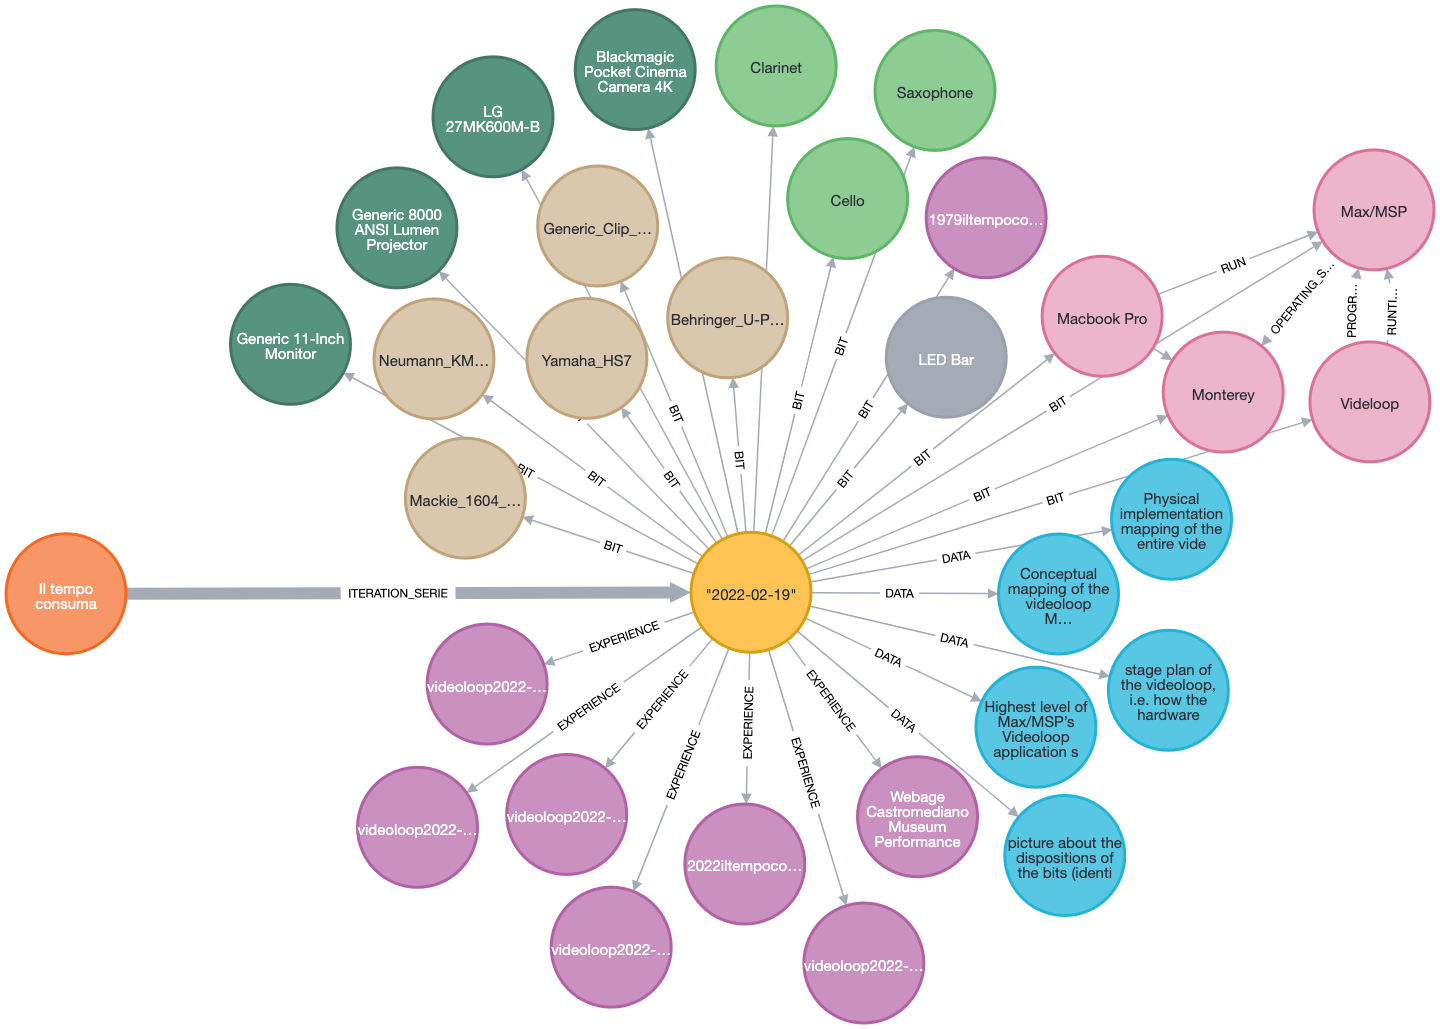
\includegraphics[width=1\linewidth]{chapters/4-MDC_model_application/image/neo4j-iteration.png}
    \caption{The relationship of an \textit{Il tempo consuma}'s iteration with \textit{bit}s, \textit{data}, and \textit{experience}.}
    \label{fig:c4-neo4j-iteration}
\end{figure}

At this level, we can see all the \textit{bit}s, such as audio components, video, hardware, and software used\footnote{In Figure~\ref{fig:c4-neo4j-iteration}, it is also possible to see the relationships between the \textit{bit}s representing the computer, operating system, and software. These relationships are enabled by the \textit{Common Information Model} (CIM), which is defined as part of the metadata standard.}; the various \textit{data}, which include all the modules and mappings related to the MIF and BVL application discussed in Chapter~\ref{ch:3-mdc_model-reactivation_workflow-instruction_template}; and finally all the experiences and the documentation created, such as a documentary video, photos, and a webpage related to the performance\footnote{In Figure~\ref{fig:c4-neo4j-iteration}, the number of collected \textit{experience}s has been significantly reduced to better visualize the database, especially in relation to other types of items.}. Therefore, when considering the MDC model, Figures~\ref{fig:c4-neo4j-artworkrelation} and ~\ref{fig:c4-neo4j-iteration} show us the \textit{multilayering} property of the model applied through Neo4j.\\
However, we still need to visualise another important property of the MDC model: \textit{multiple belongingness}. We can easily create and display this property thanks to Neo4j’s system of relationships and queries. The \textit{videoloop} case study also provides many interesting examples of \textit{multiple belongingness} in practice.\\
First, let’s start with the most superficial relationships of \textit{multiple belongingness}, which can be found at the level of \textit{bit}s and \textit{data}, such as items that belong to more than one iteration. In the context of Neo4j, we only need to create the \textit{bit} or \textit{data} item once and then create a relationship for each iteration. To visualise the relationship through Cypher, we simply need to query the database to determine which iterations use that specific item.\\
\begin{lstlisting}[style=cypher]
MATCH (i:ITERATION)-[:BIT]->(a:AUDIO_EQUIPMENT {identifier: "Behringer_U-Phoria_UMC204HD"})
\end{lstlisting}
With this simple command, we ask the database which iterations use the Behringer U-Phoria UMC204HD audio interface as a \texttt{BIT} relationship. The output is shown in Figure~\ref{fig:c4-neo4j-multiplebel01}.

\begin{figure}[!h]
    \centering
    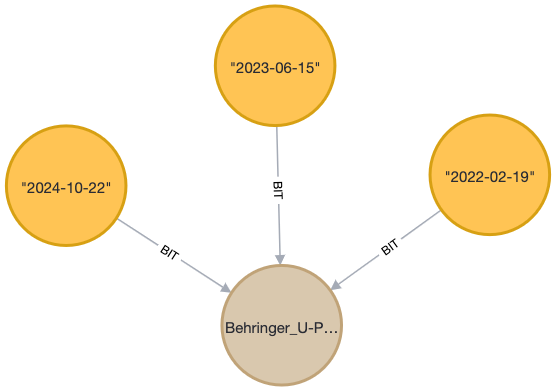
\includegraphics[width=0.5\linewidth]{chapters/4-MDC_model_application/image/neo4j-multiplebel01.png}
    \caption{\textit{Multiple Belongingness} for the audio interface Behringer U-Phoria UMC204HD in Neo4j.}
    \label{fig:c4-neo4j-multiplebel01}
\end{figure}

As we can read from the output, three iterations use this specific audio interface.\\
When analysing this artwork, another very interesting example is the usage of mappings, especially \textit{Conceptual Mapping}. As defined in Appendix~\ref{ax:a-michele_sambin_videoloop}, related to this case study, \textit{Conceptual Mapping} is the common element across all iterations, both from the 1970s and those reactivated in the digital domain. However, if we don’t already know this information, we can ask the database to find the common elements across all iterations. This kind of information can be useful for understanding whether there is a recurring element across all the iterations that could, in specific analysis, be defined as a critical element of the artwork’s identity.\\
To obtain this information, we must write a more ``complex'' Cypher query, which is still very short. First, we must match all relationships between the iteration nodes and other nodes (items). Indeed, we need to select those relationships that start from the iteration, i.e. directional relationships from the iteration to the item level (otherwise, we would obtain the artwork as common nodes).
\begin{lstlisting}[style=cypher]
MATCH (i:ITERATION)-[r]->(n)
\end{lstlisting}
Then, we must create a list aggregating all the nodes found for each iteration.
\begin{lstlisting}[style=cypher]
WITH i, COLLECT(n) AS relatedNodes
\end{lstlisting}
So, for each \texttt{ITERATION} (\texttt{i}), we will collect the related nodes (\texttt{n}), resulting in a structure like the table~\ref{tab:c4-neo4jtable01}:

\begin{table}[!h]
    \centering
    \begin{tabular}{|c|c|}
    \hline
        \textbf{\texttt{i}}  & \textbf{\texttt{relatedNodes}} \\ \hline
         1          & \texttt{[n1, n2, n3, ...]} \\ \hline
         2          & \texttt{[n3, n5, ...]} \\ \hline
         3          & \texttt{[n1, n3, n6, n7, ...]} \\ \hline
         ...          & ... \\ \hline
    \end{tabular}
    \caption{Node connected to each iteration.}
    \label{tab:c4-neo4jtable01}
\end{table}
Then, we use a series of commands to find the common nodes across the different lists (e.g., in the table above, this would be \texttt{n3}).
\begin{lstlisting}[style=cypher]
WITH COLLECT(relatedNodes) AS allRelatedNodes
WITH REDUCE(common = HEAD(allRelatedNodes), current IN TAIL(allRelatedNodes) |
    [node IN common WHERE node IN current]) AS commonNodes
\end{lstlisting}
Using the \texttt{COLLECT} command, we group all the lists of nodes from individual iterations into a single ``list of lists,'' structured as \texttt{allRelatedNodes = [[n1, n2, n3], [n3, n5], [n1, n3, n6, n7], …]}. Then, we reduce (\texttt{REDUCE}) this list to keep only the nodes that appear in every sublist. Step by step, we start with the first sublist in \texttt{allRelatedNodes} and compare it with the rest of the sublists one by one, using the commands \texttt{HEAD} (to get the first sublist) and \texttt{TAIL} (to get the remaining sublists). For each comparison, we check which nodes are shared between the current ``common'' nodes and the next sublist using \texttt{[node IN common WHERE node IN current]}. Once we’ve compared all the sublists, we get a final list of nodes shared across all sublists saved as \texttt{commonNodes}.\\
In our case, as mentioned earlier, we get the graph shown in Figure~\ref{fig:c4-neo4j-multiplebel02}.

\begin{figure}[!h]
    \centering
    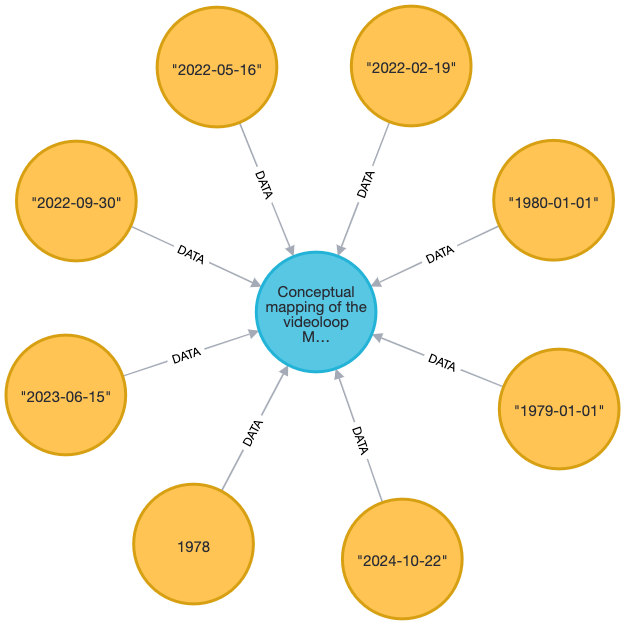
\includegraphics[width=0.75\linewidth]{chapters/4-MDC_model_application/image/neo4j-multiplebel02.png}
    \caption{Result of the search for the node common to all iterations. By querying the Neo4j database of ‘il tempo consuma’ by michele sambin (structured according to MDC) we found the concept mapping as a fixed element between iterations. This is possible due to the \textit{multiple belongingness} property of the MDC model.}
    \label{fig:c4-neo4j-multiplebel02}
\end{figure}

We can go quite far with the search for \textit{multiple belongingness}, especially in this case study. For example, we can see how an item can have two different functions for two different iterations. The video produced for the \textit{Il tempo consuma} performance in 1979 documents the same performance and is therefore classified as an \textit{experience}. However, as shown in Appendix~\ref{ax:a-michele_sambin_videoloop}, the same video is used as the introduction to the digital \textit{videoloop} performance. The digital performance of the \textit{videoloop} begins with this video recording, which dissolves into the present live performance (transitioning from the young Michele Sambin of 1979 to the present one, emphasising the time-consuming theme). So, in the reactivated versions, the video recording is considered a \textit{bit}, as shown in Figure~\ref{fig:c4-neo4j-expbit}.
\begin{figure}[!h]
    \centering
    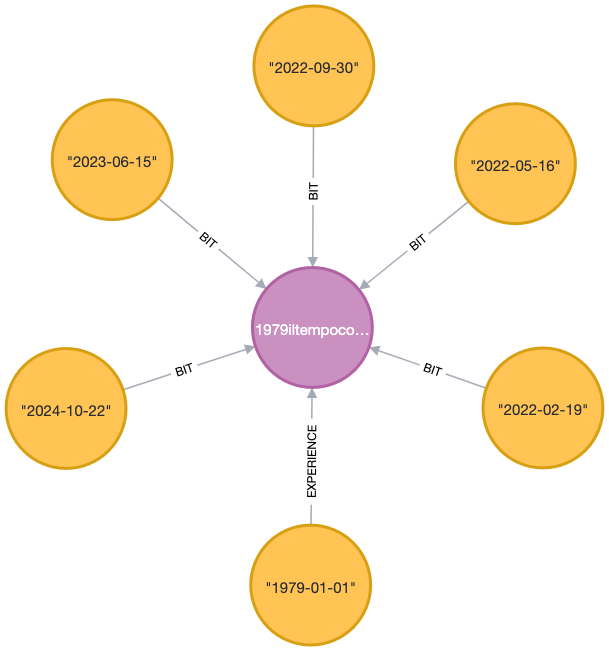
\includegraphics[width=0.75\linewidth]{chapters/4-MDC_model_application/image/neo4j-expbit.png}
    \caption{According to the \textit{Multiple Belongingness}, the same item can be associated with different iterations, each serving a different function. In this case, the \textit{videoloop} video recording remains as an \textit{experience} in one performance, while acting as a \textit{bit} in the digitally reactivated iterations.}
    \label{fig:c4-neo4j-expbit}
\end{figure}
This case is an example of reused documentation as an artistic element (documentation \textit{as art}), which we discussed in Chapter~\ref{ch:2-new_conservation_paradigms}. And this is also why, within Neo4j, we do not define items as \textit{bit}s, \textit{data}, or \textit{experiences}. Instead, we define them as items with characteristics independent of the conservation model, such as simple devices, mappings, photos, videos, etc. The quality that defines the item in the context of the MDC model—i.e., \textit{bit}, \textit{data}, and \textit{experience}—is determined by the relationship with the iteration.\\
As defined in Chapter~\ref{ch:3-mdc_model-reactivation_workflow-instruction_template}, the property of \textit{multiple belongingness} can occur not only at the lowest level of the model but also at the series level. The \textit{videoloop} is a very interesting case from this perspective because, in the reactivated versions, a series of different works are performed, not just \textit{Il tempo consuma} (see Appendix~\ref{ax:a-michele_sambin_videoloop} for more information). Therefore, if we take an iteration from the reactivations, for example, the first one in 2022 at the Castromediano Museum in Lecce, we can see that this iteration belongs to more than one artwork. In Figure~\ref{fig:c4-neo4j-multipleartworks}, we can see the \textit{multiple belongingness} of an iteration in relation to the artworks.

\begin{figure}[!h]
    \centering
    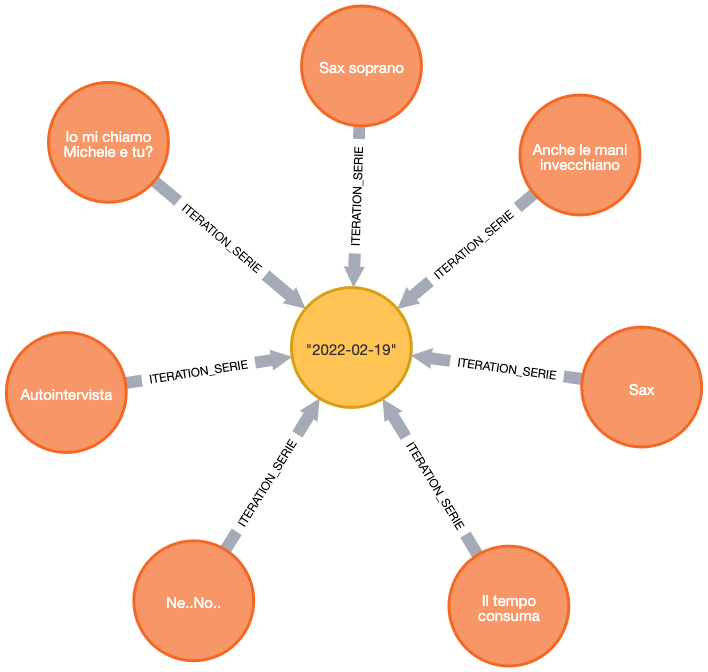
\includegraphics[width=0.75\linewidth]{chapters/4-MDC_model_application/image/neo4j-multipleartwork.png}
    \caption{According to the \textit{multiple belongingness}, even a single iteration can be associated with multiple artworks. This graph illustrates a Neo4j example of the reactivated \textit{videoloop}, where other pieces (beyond just Il tempo consuma) are performed in sequence (refer to Appendix~\ref{ax:a-michele_sambin_videoloop} for more information)}.
    \label{fig:c4-neo4j-multipleartworks}
\end{figure}

Finally, We can also see the relationship between archived artworks (i.e. those by different authors). For example, we can see the artworks exhibited in a specific event. In our case, we have an example that links the \textit{videoloop} to another reactivated artwork, \textit{Il caos delle sfere}. During the Science4all event on 30 October 2022 in Padua, both works were exhibited (the \textit{videoloop} as an installation) in the same space. In Figure~\ref{fig:c4-neo4j-event}, we can see the relationship between the two artworks through the event.

\begin{figure}[!h]
    \centering
    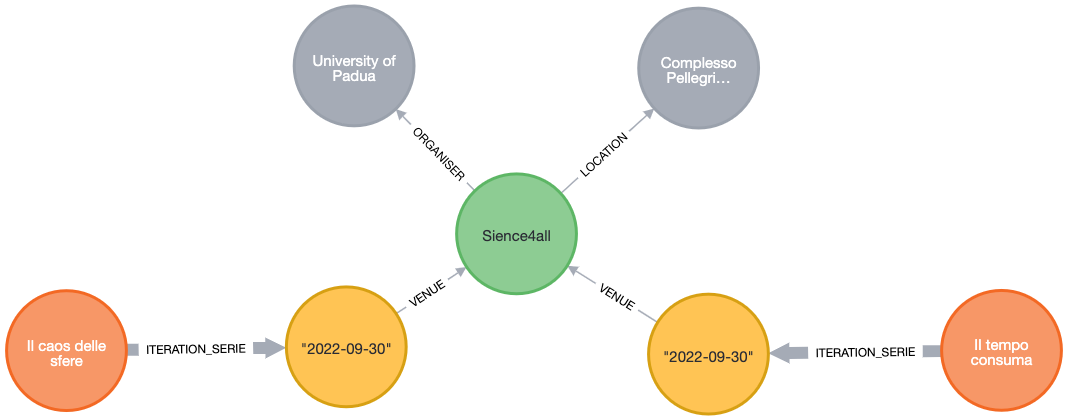
\includegraphics[width=\linewidth]{chapters/4-MDC_model_application/image/neo4j-event.png}
    \caption{Relationship between two archived artworks in the Neo4j database. The connection is traced through the reactivation of \textit{videoloop} and the installation \textit{Il caso delle sfere}, which were presented together in the same event.}
    \label{fig:c4-neo4j-event}
\end{figure}

These are just a few simple examples, but they are also very relevant in showcasing the potential of Neo4j, its Cypher query language, and the design of the MDC model in relation to this graph database.\\
The database can be used in various ways, from its use on the web, such as in an online archive, to desktop applications for both archiving and generating descriptive sheets for artworks. For example, in our case, we developed a simple Python application that can create both identity reports, similar to those used by museums, and technical sheets for further reactivations of the artwork\footnote{The python code for creating Identity Report or Technical sheets can be found in the GitHub repository of this thesis. }. 

\subsection{GitHub Repositories application}
Another application of the MDC model is through GitHub. As mentioned, GitHub is a popular web-based platform for version control and collaborative software development. It is built on Git, a distributed \textit{Version Control System} (VCS) that allows developers to track changes, manage projects, and collaborate on both open-source and private software. Git works with repositories—storage locations used to collect and manage data. One key advantage of Git compared to other VCSs is its ability to preserve a complete repository copy with full history and version tracking. Today, Git is the standard among existing VCSs, and GitHub and GitLab are the primary platforms for its use.\\
As previously discussed in this chapter and Appendix~\ref{ax:d-sustainability_and_longevity_of_nimes}, we chose to test this development platform because it is widely used in various research projects, not only scientific ones but also increasingly in artistic and creative projects. For example, it is often used in the aforementioned context of New Interfaces for Musical Expression (NIME), which is a highly interdisciplinary field combining both scientific and artistic research.\\
We applied the MDC model for archiving and documenting two NIMEs: \textit{Soundrise}, a multimedia application developed by the CSC, and \textit{Electronic\_Khipu\_} and \textit{Kanchay\_Yupana}, two complementary digital musical instruments (DMIs) created by Patricia Cadavid, a Colombian musician and researcher.\\
Before diving into the application of the MDC model in this context, some clarifications are needed. First, it is essential to emphasise that GitHub is not an archival tool. While it does have some potential for archival purposes, especially for preserving source code, tracking versions, and similar tasks, it is not specifically designed for this function. Instead, GitHub complements archival systems. For example, in the context of the Neo4j archive, GitHub could support the archiving of original software developed for the artworks. However, it is unlikely to function effectively as a standalone archival system.\\
GitHub is primarily a development tool. Its version tracking and file preservation features are aimed more at analysis, bug tracking, problem-solving, and collaborating on changes rather than long-term archiving. For instance, one key difference between GitHub and a traditional museum archive is their focus. Museum archives typically prioritise documenting the ``original'' version of an item, while GitHub (and software development in general) focuses on the ``latest version.''\\
Our specific application does not perfectly align with either case. We have moved beyond the idea of an ``original'' work, and we cannot focus solely on the ``latest version.'' Instead, we need to consider the entire set of versions. Thus, we need to adapt the design of a GitHub repository to fit the MDC model.\\
Another important aspect that differs from the Neo4j application is that GitHub is more like a ``cloud platform'' for storing files while Neo4j is just a database designed to store and manage data and could be integrated with cloud services. Although GitHub is better suited for storing source code files and text, it can also store images, audio, and videos. However, videos and large files (limited to 2GB for the free plane) cannot be directly viewed within GitHub’s web interface.\\
While GitHub lacks a dedicated tool for managing databases like Neo4j, and the case studies where the MDC model has been applied often follow different principles compared to artworks, it is still important to apply the MDC model in this context. Again, GitHub is increasingly being used in multi- and interdisciplinary fields and is more and more popular in the arts, which is why it is important to design the application of the MDC model with it.\\
\newline
A GitHub repository functions as a file storage system and includes an editable front page that serves as documentation. This page can contain textual information, images, and links related to the repository or external sources. The page is created using a \texttt{README.md} file, which works similarly to \texttt{index.html} in web pages. It can be edited using GitHub’s Markdown language (the ``.md'' extension comes from Markdown) and includes basic HTML tags.\\
We can have multiple \texttt{README.md} files, one for each directory, so each directory has its own introductory page. We can also add more \texttt{.md} files to expand the documentation for the repository or specific directories. In practice, when viewing a GitHub repository, we see the directory structure, which is displayed as folders and files, along with the front page. We can navigate through the repository or interact with the front page by reading the documentation and following the provided links.\\
In the main directory, we can also have other important files commonly used in software development and sharing. For example, a \texttt{LICENSE} file specifies the terms under which the project can be used or distributed. For each file, especially text files (such as code files), and excluding larger multimedia files (like videos), we can have specific features for viewing and interacting with the files. For instance, text files can be edited directly within GitHub.\\
The most important feature of a GitHub repository is the VCS, which allows us to track the history and changes made to the repository. Every update creates a \textit{commit}, which we can comment on to describe the changes. A \textit{commit} is a snapshot of the changes made to the repository, helping us track modifications over time. We can also create multiple branches—parallel versions of the repository. In addition to the main development branch, called ``main,'' we can develop several branches for specific development tasks or experimentation. Figure~\ref{fig:c4-github-tree} shows a typical repository development with commits and a tree of branches.

\begin{figure}[!h]
    \centering
    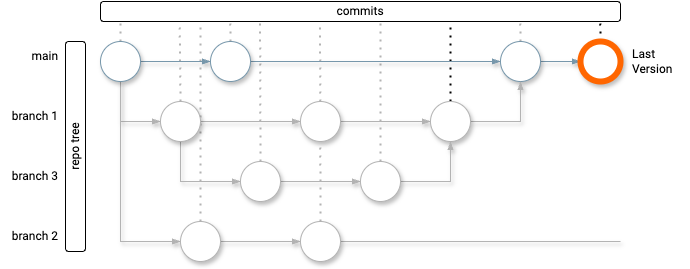
\includegraphics[width=1\linewidth]{chapters/4-MDC_model_application/image/graph04-githubtree.png}
    \caption{VCS repository development tree.}
    \label{fig:c4-github-tree}
\end{figure}

Within the \texttt{README.md} file, we can include links to different versions (based on the repository’s history) and various branches. GitHub also offers many other useful features for software development, such as collaboration tools, \textit{Issues}, \textit{Pull Requests} (PRs), and \textit{Discussions}, as well as automation, settings, and accessibility options. However, in our case, we will focus on GitHub’s essential features, which we will use primarily as a storage system.\\
We created a template repository to demonstrate the ideal application of the MDC model through GitHub. The repository is structured as shown in Figure~\ref{fig:c4-github-template}.

\begin{figure}[!h]
    \centering
    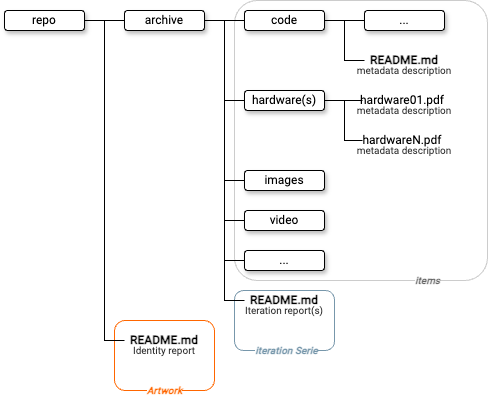
\includegraphics[width=\linewidth]{chapters/4-MDC_model_application/image/graph04-githubtemplate.png}
    \caption{GitHub repository structure template according to the MDC model appilication.}
    \label{fig:c4-github-template}
\end{figure}

The repository's main directory contains two main components: an archive subdirectory and the \texttt{README.md} file. The \texttt{README.md} serves as the general description of the artwork and follows the descriptive fields defined in the \textit{Identity Report} metadata schema. In this case, the \textit{bibliographySeries} field will be filled on the same page as the identity report, while the \textit{iterationSeries} field will refer to the \textit{archive} subdirectory. At this level, we have the highest level of the MDC model, the \textit{Creative Work} level.\\
Within the \textit{archive} subdirectory, we have additional subdirectories and, again, another \texttt{README.md}. This \texttt{README.md} will represent the \textit{Iteration Series}, which will be filled out using the \textit{Iteration Report} metadata schema. Each iteration will have a table with the main information about the iteration, followed by a set of details. The details will include \textit{bit}s, \textit{data}, and \textit{experience}. For \textit{bit}s (component list), we will use simple fields like \textit{type} (e.g., computer system, software, audiovisual), \textit{name}, \textit{version} (optional), \textit{link} (internal or external), \textit{requirements} (optional), and \textit{notes} (optional). The \textit{data} section (technical notes, mapping, and instructions) will include text and images, ideally following the instruction template defined in Chapter~\ref{ch:3-mdc_model-reactivation_workflow-instruction_template}. Finally, the \textit{experience} section (documentation) will contain photos, videos, and links to external or internal files. Figure~\ref{fig:c4-github-template02} is a schematic of the archive’s \texttt{README.md} file.

\begin{figure}[!h]
    \centering
    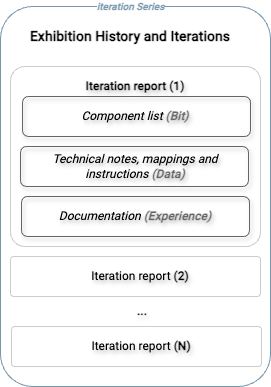
\includegraphics[width=0.4\linewidth]{chapters/4-MDC_model_application/image/graph04-githubtemplate02.png}
    \caption{GitHub repository structure template according to the MDC model appilication. Structure of the archive's \texttt{README.md} with the \textit{Creative Work}'s iterations}
    \label{fig:c4-github-template02}
\end{figure}

The subdirectories within the \textit{archive} will contain all the files related to the artwork, such as images, videos, source code, and hardware components. Following the Neo4j application approach, we do not separate \textit{bit}s, \textit{data}, and \textit{experience} at the storage level since the same item might be used differently across different iterations. The classification of an item as a \textit{bit}, \textit{data}, or \textit{experience} occurs at the iteration description level. Each item should have a proper description compiled. For source code, for example, we could have a folder containing all directories related to the specific code, organised by programming language, system used, and developer. However, here, in the main directory for the source code, we could use the \texttt{README.md} file to compile the metadata description. In other cases, such as for hardware, we could use PDFs or text files (ranging from a simple \texttt{.txt} to more specific formats like \texttt{JSON}) to compile the metadata for the specific hardware item (an example, in the template repository, is the PDF of the mechanical arm).\\
So far, we have described the hierarchical structure of the MDC model applied to a GitHub repository. Applying \textit{multiple belongingness} in this context is less effective than in Neo4j; however, it still has its potential, especially in some instances. Firstly, GitHub does not have a built-in feature to show all the pages or files directly where a specific file is referenced within a repository. This means we cannot quickly and clearly visualise \textit{multiple belongingness} as we could in Neo4j. Instead, we can only create links in the \textit{iteration series} to refer to a specific file for each iteration. This can be seen in the \textit{iteration series}’ components list under the \textit{link} field in the table. However, here, we can take advantage of one of Git’s main features: the history and branches of the repository. In the same repository, for each release of a code or specific version (for which we can create branches), direct references are automatically created, and they can be tracked. In the \texttt{README.md} files, we can refer to each step and path of the code, specifically to each commit. This allows us to avoid creating multiple copies of the same file for different versions, and instead, we can simply reference it using Git commits.\\
Below is a simple example of using this in the \textit{mdc-template} repository.\\
We start by adding the final version of the software to the repository, which will be used in the first iteration of the artwork. This action can be done through the web interface or via terminal commands. The terminal commands will look like this:
\begin{lstlisting}[style=bash]
$ git add archive/firmaware                   # add the firmware directory to the repo
$ git commit -m “firmaware-release-v1.0.0”    # commit the action as the new release
$ git commit push                             # push the new file in GitHub repo
\end{lstlisting}
The reference link used in the first and only iteration described in the README.md will be:
\begin{lstlisting}[style=markdown]
<!-- [name link](/path/to/the/folder) -->
[repo link](firmware)                          # push the new file in GitHub repo
\end{lstlisting}
Since the \texttt{README.md} and the firmware directory are in the same archive directory, we only need to enter the firmware folder. After developing a new version of the firmware, we would repeat the process and upload the latest release. This time, the commit would be:
\begin{lstlisting}[style=bash]
$ git commit -m “firmaware-release-v2.0.0”     # commit the new file in GitHub repo
\end{lstlisting}
The new iteration described in the \texttt{README.md} will have the same link as before, pointing to the latest release in the firmware directory. However, the link will change from the first release to:
\begin{lstlisting}[style=markdown]
<!-- [name link](https://github.com/example-user/repository/commit/commit_hash) -->
[commit link] (https://github.com/user/mdc-template/commit/255c12bfb5746cbc1978f076ae05f1f10b72bb51)
\end{lstlisting}
This link refers to the repository's main directory: \texttt{github.com/user/mdc-template/}. We search for a specific \textit{commit} using its hash (``commit\_hash''), which is an identifier string (e.g., \texttt{c4d2a03}). Clicking on the link will take us to the files from the first firmware version.\\
If we want to access the entire release history (and all firmware commits), we can go to the firmware’s main directory. On this page, above the \texttt{README.md} and the root of the folder, we can access the ``History'' section. Inside the History page of a specific folder or file, we can see the list of commits with their corresponding hashes. We can access different branches in the repository's main directory. Under the repository name, we can view and select different branches.\\
\newline
This application is a basic GitHub application that fits the MDC model. Of course, it can be extended to other use cases by utilising various features and capabilities of Git and GitHub.\\
We have adopted and adapted this template for the case studies introduced in Appendix~\ref{ax:d-sustainability_and_longevity_of_nimes}.\\
The \textit{Soundrise} repository was developed as a historical archive for the application and closely follows the GitHub template structure described earlier. However, there are slight differences. In this case, we are not dealing with an artwork but a web application (originally a desktop one). This difference required revising the descriptive fields (no longer the \textit{Identity Report} fields), which is the main modification compared to the template. Other changes were made, but they are of little significance (e.g., the \texttt{README.md} in the main directory includes a \textit{Technical Notes} section, as the technical aspect of the web application is essential).\\
The repository for Patricia Cadavid’s DMIs is more distant from the template. In this case, the repository’s purpose is not strictly archival but instead focused on longevity, replicability, and the continuation of the DMI. We adapted the template to a more development-oriented approach, making it more appropriate for a GitHub repository. The first revision involved removing the \textit{archive} directory, and all software and hardware components were placed in the main directory for easier access. In the same main directory, we created a documentation folder to store all video and audio documentation, as well as two other essential folders: \textit{instructions} and \textit{old\_versions}. Since the repository is focused on replicability and the continuation of the instrument, the \textit{instructions} folder (containing details about how to build the instrument) plays a central role. The \textit{old\_versions} folder contains previous iterations of the instrument. Figure~\ref{fig:c4-github-template03} shows the directory structure for Patricia Cadavid’s instruments repository.

\begin{figure}[!h]
    \centering
    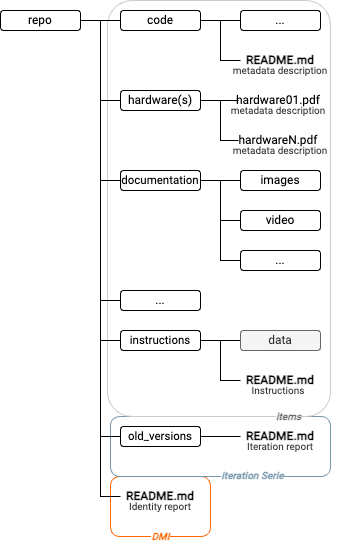
\includegraphics[width=0.75\linewidth]{chapters/4-MDC_model_application/image/graph04-github-template03.png}
    \caption{GitHub repository structure for Patricia Cadavid's digital musical instrument.}
    \label{fig:c4-github-template03}
\end{figure}

Although somewhat intricate, we have seen that the MDC model can also be applied in the context of GitHub. However, Git and GitHub are particularly suited for project development and less adaptable for archival purposes, especially when storing numerous multimedia files. For archival needs and extracting data with complex relationships, Neo4j is undoubtedly a more suitable tool. That said, in more complex and comprehensive contexts, combining Neo4j and GitHub (along with a storage system for multimedia files) creates a robust solution for implementing the MDC model. For instance, consider the DMIs developed by Cadavid. Installations or performances that use these DMIs in conjunction with other devices, multimedia files, etc., could be archived using a Neo4j database. Neo4j nodes could represent the DMIs (as \textit{bit}s) and link directly to their GitHub repositories. The GitHub repositories would contain all information about the DMIs and their development. Neo4j nodes could reference previous versions of the DMIs simply by linking to GitHub \textit{commit}s. This approach would create an interesting hierarchical relationship between two MDC archives, effectively representing the complexity of live media art projects.

\subsection{Finder management system application}
In contrast to the complexity and effectiveness of combining Neo4j and GitHub, we present the simplest and most basic application of the MDC model: using Apple’s Finder. While this method is the least likely to achieve the ideal and functional structure of the MDC model, the use of Finder (or similar local file management systems) is still crucial. In many situations, it becomes a necessary tool. In our cases, we used Finder before a more structural archiving, during the reactivation process, or for personal archiving of copyrighted works. This scenario often occurs when a work’s ``actor''—such as a performer, collaborator, or developer—needs to archive materials related to their contributions. Due to copyright restrictions, these materials are typically stored on personal computers (or, less frequently, in private cloud repositories). This scenario involves what we call an ``actor’s archive'', where an individual actor maintains a collection of their contributions (e.g., performances, software development, etc.) to enable future reactivations. An example from our work is the reactivation and performance of live electronics pieces discussed in Appendix~\ref{ax:c-the_score_in_live_electronics_music}, particularly \textit{Perseo e Andromeda}. For this piece, we gathered extensive documentation on past versions and performances, including scores, code, audio and video recordings, photos, and more. This documentation was essential for the \textit{Assessment} and \textit{Transcription} phases of the live electronics component of the piece. However, the work is subject to copyright by Ricordi, and the original materials are stored in the Paul Sacher Foundation in Basel and the Archivio Storico Ricordi in Milan. As such, we could not create a public archive; instead, we maintained all documentation locally for future reactivations.\\
When using Finder, it’s important to remember that it is a basic storage system. It only allows us to create directories (folders) and place files within them. Unlike repositories, it does not offer features like presentation pages. However, we can use two key features of Finder: \textit{Aliases} and \textit{Tags}. Figure~\ref{fig:c4-finder} shows how the MDC model can be used to organise directories in a Finder folder.

\begin{figure}[!h]
    \centering
    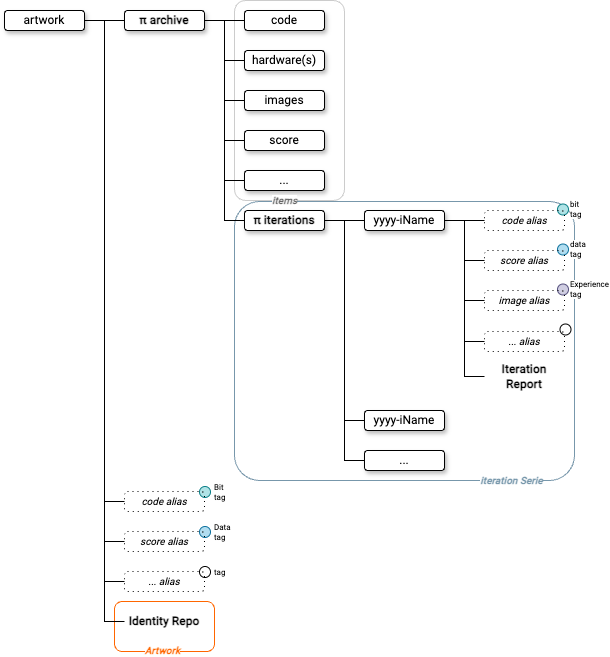
\includegraphics[width=\linewidth]{chapters/4-MDC_model_application/image/graph04-finder.png}
    \caption{A Finder folder organised according to the MDC model, using Aliases (indicated by the dotted boxes) and Tags (represented by the coloured circles in the top-right corners of the boxes).}
    \label{fig:c4-finder}
\end{figure}

This folder organisation was also used to archive \textit{Perseo e Andromeda}. First, the directories' structures are very similar to those shown in Figure~\ref{fig:c4-github-template} (in the context of the GitHub template) and Figure~\ref{fig:c4-github-template03} (in the context of Cadavid’s tool repository). The key similarity is the \textit{archive} folder, which contains all items, such as code, scores, images, videos, etc. Inside the \textit{archive} folder, there is an \textit{iterations} folder (similar to the \textit{old\_version} folder in Cadavid’s repository), where different iterations of the work are grouped into subfolders named \texttt{yyyy-iName} (year and the iteration name). Both of these folders start with the Greek letter $\pi$ (pi). This character is one of the few sorted after ``z'' in Finder’s alphabetical ordering, ensuring that the \textit{archive} and \textit{iterations} folders always appear at the bottom of the list, thus making it easier to find among the other folders.\\
The main differences compared to GitHub are the lack of the \texttt{README.md} file, the use of \textit{aliases}, and the use of \textit{tags}. Instead of \texttt{README.md}, we can use PDFs or text files (\texttt{.txt}, \texttt{.json}, etc.) created specifically for the \textit{Identity} and \textit{Iteration Reports}. However, there is a problem in linking an object to a specific iteration in which it belongs. In Neo4j, we could create direct relationships, while in GitHub, we used links in \texttt{README.md} to reference a specific object in the repository. In Finder, this relationship can be made using \textit{aliases}. An \textit{alias} is a special kind of shortcut that acts as a pointer to the original file or folder. It allows you to access or open the original item from another location without duplicating it. In Finder, you can create multiple \textit{aliases} for a file and place them in the specific iteration folder where that file belongs. Using \textit{aliases} allows us to apply the MDC model’s \textit{multiple belongingness} property.\\
To indicate the type of relationship between the iteration and a specific item, we used the iteration label in Neo4j, while in GitHub, we created a specific table listing all properties in the iteration report. In Finder, we can create and use custom \textit{tags} for files and folders. In our case, we use them only for aliases to indicate the type of relationship between the iteration and the specific alias, which can be \textit{bit}, \textit{data}, or \textit{experience}. Even here, we do not define the item type in the archive but rather its specific use within a single iteration.\\
One last point to note, which is very similar to Cadavid’s DMIs repository, is the use of \textit{aliases} in the main folder of the artwork. This type of organisation is done mainly for convenience. For example, the folder for \textit{Perseo e Andromeda} is organised to quickly access the score and the live electronics environment (code) during the redesign and implementation phases.\\
Of course, applying the MDC model through Finder is very basic but still very important. It represents what we call ``actor archiving'' and can be used for personal archiving or as a preparatory organisation before the more structured archive.  

\section{BVL adaptation}
To conclude this chapter, we introduce the adaptation of the \textit{Baalman Visual Language} (BVL) to describe mappings in the context of the free, cross-platform online application Diagram.net. As mentioned earlier in the chapter, Marija Baalman provides a dedicated GitHub repository for applying the visual language introduced in her book \textit{Composing Interaction} \cite{baalman2022composing}. This repository contains all the elements (shapes, text, fonts, arrows, etc.) defined by the language. However, we found the use of these objects to be somewhat restrictive and not very practical. For this reason, we decided to reuse the language and its main concepts within a Diagram.net. This web application is simple and intuitive to use. It requires no specific skills, allowing users to quickly create anything from basic to complex diagrams, schemes, and flowcharts. Since it is cross-platform, you can work on it from a computer, phone, or tablet. It can also be integrated with Google Drive, enabling cloud storage and real-time collaboration on shared documents. Diagram.net is an excellent tool for this kind of application, especially considering that the BVL defines only a few types of figures.\\
Below, we present our implementation using Diagram.net and compare it to the original Baalman application. For each level (see Chapter 4), we also provide simple usage examples.

\subsection{Conceptual Level}
For the \textit{Conceptual Level}, the BVL uses only five elements: \textit{actor}, \textit{physical elements}, \textit{concept clarifications}, \textit{action}, and \textit{effect}. Table~\ref{tab:c4-bvl_conceptual} shows that the visual design of the original version and the adaptation in Diagram.net are very similar.

\begin{longtable}{|m{0.18\textwidth}|m{0.18\textwidth}|m{0.55\textwidth}|}
    \caption{Adaptation of BVL boxes to \textit{Conceptual Level}} \label{tab:c4-bvl_conceptual} \\
    \hline
    \textbf{Original} & \textbf{Adapted} & \textbf{Description} \\
    \hline
    %%%%%%%%%%%%%%%%%%%%%%%%%%%%%%%%%%%%%%%%%%%%%%%%%%%%%%%%%%%%%%%%%%%%%%%%%%%%%%%%%%%%%%%%%%%%%%%%%%%%
    \centering
    
\includegraphics[width=0.75\linewidth]{chapters/4-MDC_model_application/image/bvl-actor-o.png}
    &
    \centering
    
\includegraphics[width=0.75\linewidth]{chapters/4-MDC_model_application/image/bvl-actor.png}
    & 
    The \textit{actor} is represented by a dashed circle with the actor's name in the centre. The circle represents the performer, the audience, the environment, or other external factors interacting with the artwork through ‘gestures’. The actor can be extended with further details. For example, a performer can be represented by two other actor elements representing both hands. Additional information can also be added through text next to the circle. 
    \\\hline
    %%%%%%%%%%%%%%%%%%%%%%%%%%%%%%%%%%%%%%%%%%%%%%%%%%%%%%%%%%%%%%%%%%%%%%%%%%%%%%%%%%%%%%%%%%%%%%%%%%%%
    %%%%%%%%%%%%%%%%%%%%%%%%%%%%%%%%%%%%%%%%%%%%%%%%%%%%%%%%%%%%%%%%%%%%%%%%%%%%%%%%%%%%%%%%%%%%%%%%%%%%
    \centering
    
\includegraphics[width=0.75\linewidth]{chapters/4-MDC_model_application/image/bvl-physicalelement-o.png}
    &
    \centering
    
\includegraphics[width=0.75\linewidth]{chapters/4-MDC_model_application/image/bvl-physicalelement.png}
    & 
    The \textit{physical} element is represented by a solid circle with the element's name in the centre. It represents the physical \textit{bit} (e.g., hardware) with which the actor interacts. Text next to the circle can also provide further information.
    \\\hline
    %%%%%%%%%%%%%%%%%%%%%%%%%%%%%%%%%%%%%%%%%%%%%%%%%%%%%%%%%%%%%%%%%%%%%%%%%%%%%%%%%%%%%%%%%%%%%%%%%%%%
    %%%%%%%%%%%%%%%%%%%%%%%%%%%%%%%%%%%%%%%%%%%%%%%%%%%%%%%%%%%%%%%%%%%%%%%%%%%%%%%%%%%%%%%%%%%%%%%%%%%%
    \centering
    
\includegraphics[width=0.75\linewidth]{chapters/4-MDC_model_application/image/bvl-action-o.png}
    &
    \centering
    
\includegraphics[width=0.75\linewidth]{chapters/4-MDC_model_application/image/bvl-action.png}
    & 
    The \textit{action} is represented by a dashed triangle pointing to the right and with the name of the specific action in the centre. The element represents the action (or gesture) produced by the actor. It can be used with the actor (``press'' a button) or with the physical element (e.g. the bow ``move'' in the cello’s string). Further information can also be added through text next to the circle.
    \\\hline
    %%%%%%%%%%%%%%%%%%%%%%%%%%%%%%%%%%%%%%%%%%%%%%%%%%%%%%%%%%%%%%%%%%%%%%%%%%%%%%%%%%%%%%%%%%%%%%%%%%%%
    %%%%%%%%%%%%%%%%%%%%%%%%%%%%%%%%%%%%%%%%%%%%%%%%%%%%%%%%%%%%%%%%%%%%%%%%%%%%%%%%%%%%%%%%%%%%%%%%%%%%
    \centering
    
\includegraphics[width=0.75\linewidth]{chapters/4-MDC_model_application/image/bvl-effect-o.png}
    &
    \centering
    
\includegraphics[width=0.75\linewidth]{chapters/4-MDC_model_application/image/bvl-effect.png}
    & 
    The \textit{effect} element is represented by a dashed rhombus with the name (or brief explanation) of the element in the centre. The \textit{effect} should always be at the end of the chain, explaining the effect (the result) produced by the same chain, i.e. by the artwork.
    \\\hline
    %%%%%%%%%%%%%%%%%%%%%%%%%%%%%%%%%%%%%%%%%%%%%%%%%%%%%%%%%%%%%%%%%%%%%%%%%%%%%%%%%%%%%%%%%%%%%%%%%%%%
    %%%%%%%%%%%%%%%%%%%%%%%%%%%%%%%%%%%%%%%%%%%%%%%%%%%%%%%%%%%%%%%%%%%%%%%%%%%%%%%%%%%%%%%%%%%%%%%%%%%%
    \centering
    
\includegraphics[width=0.75\linewidth]{chapters/4-MDC_model_application/image/bvl-concept-o.png}
    &
    \centering
    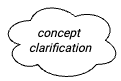
\includegraphics[width=0.75\linewidth]{chapters/4-MDC_model_application/image/bvl-concept.png}
    & 
    The \textit{concept clarification} element is represented by a solid cloud with a short text explaining the concept in the centre. This element enhances the information about the described concept and is usually placed near the \textit{action} or \textit{effect} elements. While the other elements are linked between them, this element is used without a link and placed near the element (or group of elements) that necessitates an in-depth explanation
    \\\hline
    %%%%%%%%%%%%%%%%%%%%%%%%%%%%%%%%%%%%%%%%%%%%%%%%%%%%%%%%%%%%%%%%%%%%%%%%%%%%%%%%%%%%%%%%%%%%%%%%%%%%
\end{longtable}

Except for the \textit{concept clarification} element, all other elements are connected by directional arrows to show the flow of actions and elements. In our implementation, we also include text above or below the links to provide more details about the relationships (e.g., the \textit{Conceptual Mapping} of Michele Sambin’s video loop in Figure~\ref{}). Finally, as mentioned earlier, the \textit{effect} element represents the output of the flowchart.\\
In Figure~\ref{fig:c4-conceptual_level} below, we present an example of a \textit{Conceptual Mapping} flow diagram created by Baalman in her book, recreated using our implementation.
\begin{figure}[!h]
    \centering
    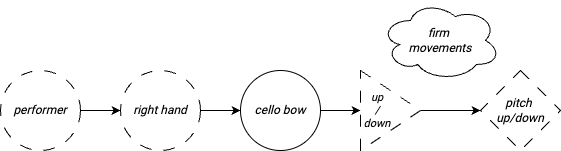
\includegraphics[width=1\linewidth]{chapters/4-MDC_model_application/image/bvl-conceptual_level.png}
    \caption{BVL application for \textit{Conceptual Mapping}. The mapping is proposed in \cite{baalman2022composing}.}
    \label{fig:c4-conceptual_level}
\end{figure}
This diagram illustrates a simple interaction where a performer can change the pitch of a cello by moving the bow (held in their right hand) vertically with firm movements, either upward or downward.\\
In this text, we have examined several conceptual mappings, starting with the introduction of the BVL in Chapter~\ref{ch:3-mdc_model-reactivation_workflow-instruction_template} (Figure~\ref{fig:c3-BVLconceptual}) and throughout the appendices (Appendix~\ref{ax:a-michele_sambin_videoloop}, Figure~\ref{}; Appendix~\ref{ax:b-hybrid_reactivation_il_caos_delle_sfere}, Figure~\ref{}; and Appendix~\ref{ax:d-sustainability_and_longevity_of_nimes}, Figure~\ref{}). All these \textit{Conceptual Mappings} describe different scenarios, yet they can be easily explained using these essential elements.

\subsection{Physical implementation Level}
The \textit{Physical Implementation Mapping} describes what happens between the gesture and the output, focusing specifically on the ``physical'' level, including various interfaces, hardware, and software. In this context, we need to define four main elements, three types of connections, and six types of streams. Table~\ref{tab:c4-bvl_physical} define the adaptation of the four main elements.

\begin{longtable}{|m{0.18\textwidth}|m{0.18\textwidth}|m{0.55\textwidth}|}
    \caption{Adaptation of BVL boxes to \textit{Physical Implementation Level}} \label{tab:c4-bvl_physical} \\
    \hline
    \textbf{Original} & \textbf{Adapted} & \textbf{Description} \\
    \hline
    %%%%%%%%%%%%%%%%%%%%%%%%%%%%%%%%%%%%%%%%%%%%%%%%%%%%%%%%%%%%%%%%%%%%%%%%%%%%%%%%%%%%%%%%%%%%%%%%%%%%
    \centering
    
\includegraphics[width=0.75\linewidth]{chapters/4-MDC_model_application/image/bvl-interface-o.png}
    &
    \centering
    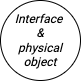
\includegraphics[width=0.75\linewidth]{chapters/4-MDC_model_application/image/bvl-interface.png}
    & 
    The \textit{interface \& physical object} is represented by a solid circle with the element's name in the centre. This element represents the physical element with which the interaction occurs. Further information can also be added through text next to the circle.
    \\\hline
    %%%%%%%%%%%%%%%%%%%%%%%%%%%%%%%%%%%%%%%%%%%%%%%%%%%%%%%%%%%%%%%%%%%%%%%%%%%%%%%%%%%%%%%%%%%%%%%%%%%%
    %%%%%%%%%%%%%%%%%%%%%%%%%%%%%%%%%%%%%%%%%%%%%%%%%%%%%%%%%%%%%%%%%%%%%%%%%%%%%%%%%%%%%%%%%%%%%%%%%%%%
    \centering
    
\includegraphics[width=0.75\linewidth]{chapters/4-MDC_model_application/image/bvl-hardware-o.png}
    &
    \centering
    
\includegraphics[width=0.75\linewidth]{chapters/4-MDC_model_application/image/bvl-hardware.png}
    & 
    The \textit{hardware} is represented by a solid square with the name of the specific hardware in the centre. This element represents any kind of hardware. Further information can also be added through text next to the square.
    \\\hline
    %%%%%%%%%%%%%%%%%%%%%%%%%%%%%%%%%%%%%%%%%%%%%%%%%%%%%%%%%%%%%%%%%%%%%%%%%%%%%%%%%%%%%%%%%%%%%%%%%%%%
    %%%%%%%%%%%%%%%%%%%%%%%%%%%%%%%%%%%%%%%%%%%%%%%%%%%%%%%%%%%%%%%%%%%%%%%%%%%%%%%%%%%%%%%%%%%%%%%%%%%%
    \centering
    
\includegraphics[width=0.75\linewidth]{chapters/4-MDC_model_application/image/bvl-software-o.png}
    &
    \centering
    
\includegraphics[width=0.75\linewidth]{chapters/4-MDC_model_application/image/bvl-software.png}
    & 
    The \textit{software} is represented by a dashed square with the name of the specific software in the centre. This element represents any kind of software. Further information can also be added through text next to the square.
    \\\hline
    %%%%%%%%%%%%%%%%%%%%%%%%%%%%%%%%%%%%%%%%%%%%%%%%%%%%%%%%%%%%%%%%%%%%%%%%%%%%%%%%%%%%%%%%%%%%%%%%%%%%
    %%%%%%%%%%%%%%%%%%%%%%%%%%%%%%%%%%%%%%%%%%%%%%%%%%%%%%%%%%%%%%%%%%%%%%%%%%%%%%%%%%%%%%%%%%%%%%%%%%%%
    \centering
    
\includegraphics[width=0.75\linewidth]{chapters/4-MDC_model_application/image/bvl-output-o.png}
    &
    \centering
    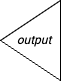
\includegraphics[width=0.75\linewidth]{chapters/4-MDC_model_application/image/bvl-output.png}
    & 
    The \textit{output} is represented by a solid triangle pointing to the left, with the name of the specific output in the centre. This element represents the system's output. It should be used at the end of the entire \textit{Physical Implementation Mapping}. Text next to the triangle can also provide further information.
    \\\hline
    %%%%%%%%%%%%%%%%%%%%%%%%%%%%%%%%%%%%%%%%%%%%%%%%%%%%%%%%%%%%%%%%%%%%%%%%%%%%%%%%%%%%%%%%%%%%%%%%%%%%
\end{longtable}

These elements are connected in order to define the flow of the physical implementation. Unlike conceptual mapping, this level involves different types of communication, represented by three types of connections that can be either unidirectional or multidirectional. The connections are:

\begin{longtable}{|m{0.1\textwidth}|m{0.49\textwidth}|m{0.32\textwidth}|}
    \caption{Adaptation of BVL connection arrow for the \textit{Physical Implementation Level}} \label{tab:c4-bvl_physical_arrow} \\
    \hline
    \textbf{} & \textbf{Type of connection} & \textbf{Description} \\
    \hline
    %%%%%%%%%%%%%%%%%%%%%%%%%%%%%%%%%%%%%%%%%%%%%%%%%%%%%%%%%%%%%%%%%%%%%%%%%%%%%%%%%%%%%%%%%%%%%%%%%%%%
    %%%%%%%%%%%%%%%%%%%%%%%%%%%%%%%%%%%%%%%%%%%%%%%%%%%%%%%%%%%%%%%%%%%%%%%%%%%%%%%%%%%%%%%%%%%%%%%%%%%%
    \centering
    \small \textbf{Original} \rule{0pt}{1.25cm} & 
    \centering
    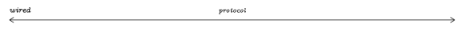
\includegraphics[width=1\linewidth]{chapters/4-MDC_model_application/image/bvl-arrow-wired-o.png} &
    \multirow{2}{*}{\parbox[t]{\linewidth}{\vspace{-1cm}The \textit{wired} connection is represented by a directional solid line. The type of connection used for the link replaces the ``protocol'' word (e.g. Audio, USB, etc.).}}
    \\
    \centering
    \small \textbf{Adapted} \rule{0pt}{1.25cm} &
    \centering
    
\includegraphics[width=1\linewidth]{chapters/4-MDC_model_application/image/bvl-arrow-wired.png} & 
    \\
    \hline
    %%%%%%%%%%%%%%%%%%%%%%%%%%%%%%%%%%%%%%%%%%%%%%%%%%%%%%%%%%%%%%%%%%%%%%%%%%%%%%%%%%%%%%%%%%%%%%%%%%%%
    %%%%%%%%%%%%%%%%%%%%%%%%%%%%%%%%%%%%%%%%%%%%%%%%%%%%%%%%%%%%%%%%%%%%%%%%%%%%%%%%%%%%%%%%%%%%%%%%%%%%
    \centering
    \small \textbf{Original} \rule{0pt}{1.43cm} & 
    \centering
    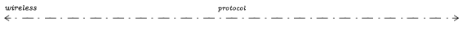
\includegraphics[width=1\linewidth]{chapters/4-MDC_model_application/image/bvl-arrow-wireless-o.png} &
    \multirow{2}{*}{\parbox[t]{\linewidth}{\vspace{-1.05cm}The \textit{wireless} connection is represented by a directional dotted line (originally by a dash-dotted line). The protocol type replaces the ``protocol'' word (e.g. Wi-Fi, Bluetooth, etc.).}}
    \\
    \centering
    \small \textbf{Adapted} \rule{0pt}{1.43cm} &
    \centering
    
\includegraphics[width=1\linewidth]{chapters/4-MDC_model_application/image/bvl-arrow-wireless.png} & 
    \\
    \hline
    %%%%%%%%%%%%%%%%%%%%%%%%%%%%%%%%%%%%%%%%%%%%%%%%%%%%%%%%%%%%%%%%%%%%%%%%%%%%%%%%%%%%%%%%%%%%%%%%%%%%
    %%%%%%%%%%%%%%%%%%%%%%%%%%%%%%%%%%%%%%%%%%%%%%%%%%%%%%%%%%%%%%%%%%%%%%%%%%%%%%%%%%%%%%%%%%%%%%%%%%%%
    \centering
    \small \textbf{Original} \rule{0pt}{1.25cm} & 
    \centering
    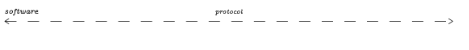
\includegraphics[width=1\linewidth]{chapters/4-MDC_model_application/image/bvl-arrow-software-o.png} &
    \multirow{2}{*}{\parbox[t]{\linewidth}{\vspace{-1cm}The \textit{software} connection is represented with a directional dashed line. It is usually used between hardware and software to indicate which hardware runs a specific software.}}
    \\
    \centering
    \small \textbf{Adapted} \rule{0pt}{1.25cm} &
    \centering
    
\includegraphics[width=1\linewidth]{chapters/4-MDC_model_application/image/bvl-arrow-software.png} & 
    \\
    \hline
    %%%%%%%%%%%%%%%%%%%%%%%%%%%%%%%%%%%%%%%%%%%%%%%%%%%%%%%%%%%%%%%%%%%%%%%%%%%%%%%%%%%%%%%%%%%%%%%%%%%%
\end{longtable}

Furthermore, this connection can have six different types of streams. The types are adapted with just a series of characters and should be placed above the connection at the beginning. The types of streams are shown in Table~\ref{tab:c4-bvl_physical_strem}

\begin{longtable}{|m{0.05\textwidth}|m{0.05\textwidth}|m{0.81\textwidth}|}
    \caption{Adaptation of BVL streams for \textit{Physical Implementation Level}} \label{tab:c4-bvl_physical_strem} \\
    \hline
    \textbf{Ori.} & \textbf{Ada.} & \textbf{Description} \\
    \hline
    %%%%%%%%%%%%%%%%%%%%%%%%%%%%%%%%%%%%%%%%%%%%%%%%%%%%%%%%%%%%%%%%%%%%%%%%%%%%%%%%%%%%%%%%%%%%%%%%%%%%
    \centering
    
\includegraphics[width=0.75\linewidth]{chapters/4-MDC_model_application/image/bvl-audio-o.png}
    &
    \centering
    
\includegraphics[width=0.75\linewidth]{chapters/4-MDC_model_application/image/bvl-audio.png}
    & 
    The \textit{Audio} stream is represented by the tilde character ($\sim$).
    \\\hline
    %%%%%%%%%%%%%%%%%%%%%%%%%%%%%%%%%%%%%%%%%%%%%%%%%%%%%%%%%%%%%%%%%%%%%%%%%%%%%%%%%%%%%%%%%%%%%%%%%%%%
    %%%%%%%%%%%%%%%%%%%%%%%%%%%%%%%%%%%%%%%%%%%%%%%%%%%%%%%%%%%%%%%%%%%%%%%%%%%%%%%%%%%%%%%%%%%%%%%%%%%%
    \centering
    
\includegraphics[width=0.75\linewidth]{chapters/4-MDC_model_application/image/bvl-video-o.png}
    &
    \centering
    
\includegraphics[width=0.75\linewidth]{chapters/4-MDC_model_application/image/bvl-video.png}
    & 
    The \textit{video} stream is represented by the open and closed square bracket with a space in between ([ ]). 
    \\\hline
    %%%%%%%%%%%%%%%%%%%%%%%%%%%%%%%%%%%%%%%%%%%%%%%%%%%%%%%%%%%%%%%%%%%%%%%%%%%%%%%%%%%%%%%%%%%%%%%%%%%%
    %%%%%%%%%%%%%%%%%%%%%%%%%%%%%%%%%%%%%%%%%%%%%%%%%%%%%%%%%%%%%%%%%%%%%%%%%%%%%%%%%%%%%%%%%%%%%%%%%%%%
    \centering
    
\includegraphics[width=0.75\linewidth]{chapters/4-MDC_model_application/image/bvl-data-o.png}
    &
    \centering
    
\includegraphics[width=0.75\linewidth]{chapters/4-MDC_model_application/image/bvl-data.png}
    & 
    The \textit{data} stream is represented by the pipe characters (\textbar) and the capital o (\textbar O).
    \\\hline
    %%%%%%%%%%%%%%%%%%%%%%%%%%%%%%%%%%%%%%%%%%%%%%%%%%%%%%%%%%%%%%%%%%%%%%%%%%%%%%%%%%%%%%%%%%%%%%%%%%%%
    %%%%%%%%%%%%%%%%%%%%%%%%%%%%%%%%%%%%%%%%%%%%%%%%%%%%%%%%%%%%%%%%%%%%%%%%%%%%%%%%%%%%%%%%%%%%%%%%%%%%
    \centering
    
\includegraphics[width=0.75\linewidth]{chapters/4-MDC_model_application/image/bvl-event-o.png}
    &
    \centering
    
\includegraphics[width=0.75\linewidth]{chapters/4-MDC_model_application/image/bvl-event.png}
    & 
    The \textit{event} stream is represented by the capital slashed o character (\O).
    \\\hline
    %%%%%%%%%%%%%%%%%%%%%%%%%%%%%%%%%%%%%%%%%%%%%%%%%%%%%%%%%%%%%%%%%%%%%%%%%%%%%%%%%%%%%%%%%%%%%%%%%%%%
    %%%%%%%%%%%%%%%%%%%%%%%%%%%%%%%%%%%%%%%%%%%%%%%%%%%%%%%%%%%%%%%%%%%%%%%%%%%%%%%%%%%%%%%%%%%%%%%%%%%%
    \centering
    
\includegraphics[width=0.75\linewidth]{chapters/4-MDC_model_application/image/bvl-buffer-o.png}
    &
    \centering
    \includegraphics[width=0.75\linewidth]{chapters/4-MDC_model_application/image/bvl-buffer.png}
    & 
    The buffer stream is represented by four pipe characters (\textbar\textbar\textbar\textbar).
    \\\hline
    %%%%%%%%%%%%%%%%%%%%%%%%%%%%%%%%%%%%%%%%%%%%%%%%%%%%%%%%%%%%%%%%%%%%%%%%%%%%%%%%%%%%%%%%%%%%%%%%%%%%
    %%%%%%%%%%%%%%%%%%%%%%%%%%%%%%%%%%%%%%%%%%%%%%%%%%%%%%%%%%%%%%%%%%%%%%%%%%%%%%%%%%%%%%%%%%%%%%%%%%%%
    \centering
    \includegraphics[width=0.75\linewidth]{chapters/4-MDC_model_application/image/bvl-spectral-o.png}
    &
    \centering
    \includegraphics[width=0.75\linewidth]{chapters/4-MDC_model_application/image/bvl-spectral.png}
    & 
    The spectral stream is represented by the lozenge (or Diamond) character ($\lozenge$).
    \\\hline
    %%%%%%%%%%%%%%%%%%%%%%%%%%%%%%%%%%%%%%%%%%%%%%%%%%%%%%%%%%%%%%%%%%%%%%%%%%%%%%%%%%%%%%%%%%%%%%%%%%%%
\end{longtable}
We can include text for each element and connection to provide additional details or explanations.
Figure~\ref{fig:c4-physical_level} presents a straightforward example of a \textit{Physical Implementation Mapping} diagram using our implementation of the BVL created with Diagram.net. This example shows a basic setup in which a sound card is connected to a computer running Max/MSP, a microphone (the interaction \textit{interface}), and a speaker (the \textit{output}).\\
For elements like \textit{Interface \& Physical Object}, and \textit{Hardware}, we can add more detailed information, such as the type and name of the input or output devices. In Figure~\ref{fig:c4-physical_level02}, we see two examples: the Adafruit BNO085, a motion sensor with an integrated accelerometer, gyroscope, and magnetometer, and an audio mixer with various types of audio inputs and outputs.\\
\begin{minipage}[t]{0.45\textwidth}
    \centering
    \includegraphics[width=\linewidth]{chapters/4-MDC_model_application/image/bvl-physical_level.png}
    \captionof{figure}{Simple BVL application for \textit{Physical Implementation Mapping}.}
    \label{fig:c4-physical_level}
\end{minipage}%
\hfill
\begin{minipage}[t]{0.45\textwidth}
    \centering
    \includegraphics[width=\linewidth]{chapters/4-MDC_model_application/image/bvl-physical_level02.png}
    \captionof{figure}{\textit{Interface \& Physical Object} (above), and \textit{Hardware} (below) examples with input and output details.}
    \label{fig:c4-physical_level02}
\end{minipage}
\newline
In this text, we have examined many \textit{Physical Implementation Mappings}, starting with the introduction of the BVL in Chapter~\ref{ch:3-mdc_model-reactivation_workflow-instruction_template} (Figure~\ref{fig:c3-BVLphysical}) and throughout the appendices (Appendix~\ref{ax:a-michele_sambin_videoloop}, Figure~\ref{}; Appendix~\ref{ax:b-hybrid_reactivation_il_caos_delle_sfere}, Figures~\ref{}, \ref{}, and \ref{}; and Appendix~\ref{ax:d-sustainability_and_longevity_of_nimes}, Figure~\ref{}).

\subsection{Process Level}
\textit{Process Mapping} involves a potentially infinite set of blocks that can be organised to describe, at a computational level, what happens between a gesture and the output—how one type of data is transformed into another. This description can be provided at different levels of detail, corresponding to various types of operations, ranging from low-level tasks (e.g., addition or subtraction) to higher-level processes (e.g., resampling).\\
The level of detail required depends on several factors, such as the complexity of the work, the need for detail (e.g., it may not be necessary to describe a low-pass filter in full detail), and practical considerations like the time, resources, and personnel available. Striking the right balance between description complexity and feasibility is not always straightforward, and in many cases, achieving a highly detailed level of description may not be possible.\\
The BVL defines a limited set of blocks, which are insufficient based on our applications. To address this, we propose an extended system within the context of our implementation. This system includes two block types: the \textit{Operation} and \textit{Function} blocks, which can be adapted to specific operations and processes.
While the \textit{Operation} block simply describes a defined operation, the \textit{Function} block describes a new process through a series of operations. The \textit{Function} block encapsulates another process that can be described using a separate \textit{Process Mapping}. This nested system can contain additional \textit{Function} blocks, creating a matryoshka-like structure. This approach helps simplify individual mappings, which might otherwise become overly complex and difficult to read.

\begin{longtable}{|m{0.30\textwidth}|m{0.68\textwidth}|}
    \caption{Adaptation of BVL blocks to the \textit{Process Level}} \label{tab:c4-bvl_process} \\
    \hline
    \textbf{Block} & \textbf{Description} \\
    \hline
    %%%%%%%%%%%%%%%%%%%%%%%%%%%%%%%%%%%%%%%%%%%%%%%%%%%%%%%%%%%%%%%%%%%%%%%%%%%%%%%%%%%%%%%%%%%%%%%%%%%%
    \centering
    \includegraphics[width=0.5\linewidth]{chapters/4-MDC_model_application/image/bvl-operation.png}
    & 
    The \textit{Operation Block} (\textit{Op. Block}) allow us to define a custom operation in the process mapping. It is represented by a square with the symbol of the operation in the centre (\$), which has to be replaced with the custom operation symbol. In the left-bottom corner, we have the extended name of the operation (\textit{Op. Block}), abbreviated if it is too long. On the left side, we have a series of defined inputs (\textit{inN}) and on the right side, a series of defined outputs (\textit{outN}), while at the top, we can have a series of arrows that define \textit{external factors}. We have a short description of the custom operation block below the box.
    \\\hline
    %%%%%%%%%%%%%%%%%%%%%%%%%%%%%%%%%%%%%%%%%%%%%%%%%%%%%%%%%%%%%%%%%%%%%%%%%%%%%%%%%%%%%%%%%%%%%%%%%%%%
    %%%%%%%%%%%%%%%%%%%%%%%%%%%%%%%%%%%%%%%%%%%%%%%%%%%%%%%%%%%%%%%%%%%%%%%%%%%%%%%%%%%%%%%%%%%%%%%%%%%%
    \centering
    \includegraphics[width=0.75\linewidth]{chapters/4-MDC_model_application/image/bvl-function.png}
    & 
    The \textit{Function block} (\textit{Function}) allows us to create custom functions. Functions are abstractions of a part of the \textit{Process Mapping} and help keep the process clear and readable. A function is represented by a rectangular shape with the function's name at the centre, a series of defined inputs and outputs on the sides, a series of defined initialisation arguments, and a short description below the shape.
    \\\hline
    %%%%%%%%%%%%%%%%%%%%%%%%%%%%%%%%%%%%%%%%%%%%%%%%%%%%%%%%%%%%%%%%%%%%%%%%%%%%%%%%%%%%%%%%%%%%%%%%%%%%
\end{longtable}
With the \textit{Operation} block, we can create custom operations, such as those presented in the Baalmans’ book \cite{baalman2022composing} (Figure~\ref{fig:c4-process_level}).
\begin{figure}[!h]
    \centering
    \includegraphics[width=1\linewidth]{chapters/4-MDC_model_application/image/bvl-process_level.png}
    \caption{Example of \textit{Operation} Block, constructed using the method above. Some of them are extracted from \cite{baalman2022composing}.}
    \label{fig:c4-process_level}
\end{figure}
The different components used to describe an \textit{Operation} block are always optional. For example, the \textit{Range} block does not include a symbol. In other cases, the symbol can be expanded—such as in the \textit{Gate} block—to represent the block's functionality better.\\
The \textit{Function} block allows us to simplify the mapping of a specific process, making it easier to read and understand. For example, consider the mapping in Figure~\ref{fig:c4-process_mapping02}.
\begin{figure}[!h]
    \centering
    \includegraphics[width=0.7\linewidth]{chapters/4-MDC_model_application/image/bvl-process_level02.png}
    \caption{An example of Process mapping using a \textit{Function} block. To simplify the mapping. Figure~\ref{fig:c4-process_level03} represent the process inscribed inside the Function block \textit{Simple Pedometer}.}
    \label{fig:c4-process_level02}
\end{figure}
In this straightforward example, the mapping is easy to read. It illustrates that light is switched on for each step detected by a pedometer (which uses the three axes of an accelerometer as input). The \textit{Function} Block \textit{Simple Pedometer} serves as an abstraction, encapsulating a more detailed process mapping. This abstraction simplifies the main mapping, making it easier to read. The \textit{Simple Pedometer} can be expanded into the detailed mapping in Figure~\ref{fig:c4-process_level03}. This mapping represents the pedometer process, which, if included in the mapping from the previous figure, would have made the entire process significantly more complex to read.
\begin{figure}[!h]
    \centering
    \includegraphics[width=\linewidth]{chapters/4-MDC_model_application/image/bvl-process_level03.png}
    \caption{The \textit{Process mapping} of a pedometer. This process was inscribed inside the \textit{Function} block \textit{Simple Pedometer} in Figure~\ref{fig:c4-process_level02}.}
    \label{fig:c4-process_level03}
\end{figure}
Furthermore, the last mapping in Fgure~\ref{fig:c4-process_level03} presents a new type of block (Figure~\ref{fig:c4-bvl-buffer}). 
\begin{figure}[!h]
    \centering
    \includegraphics[width=0.2\linewidth]{chapters/4-MDC_model_application/image/bvl-bufferblock.png}
    \caption{The \textit{Process Mapping}'s \textit{Buffer} block.}
    \label{fig:c4-bvl-buffer}
\end{figure}
This block type can describe a sequence of numbers or bits, such as arrays or buffers. In previous mappings (Figures~\ref{fig:c4-process_level02} and \ref{fig:c4-process_level03}), we also see the \textit{Interface & Physical Objects} block, which can be used to define input data more precisely. Similarly, the Output block can specify the output type in greater detail.
In process mapping, we can generally incorporate all other types of objects defined at higher levels to better clarify and contextualise the process.\\
In this text, we have examined many \textit{Process Mappings}, starting with the introduction of the BVL in Chapter~\ref{ch:3-mdc_model-reactivation_workflow-instruction_template} (Figure~\ref{fig:c3-BVLprocess}) and throughout the appendices (Appendix~\ref{ax:a-michele_sambin_videoloop}, Figure~\ref{}; Appendix~\ref{ax:b-hybrid_reactivation_il_caos_delle_sfere}, Figures~\ref{}; and Appendix~\ref{ax:d-sustainability_and_longevity_of_nimes}, Figure~\ref{}).

\section{Summary}
In this chapter, we demonstrated how to apply the MDC model on three different platforms: 1) using the Neo4j graph database, 2) using the GitHub development platform, and 3) using Apple’s Finder file management system. These applications highlight the model’s adaptability to various use cases and levels of complexity: 1) a more extensive, comprehensive application that could reflect the needs of a web-based or private archive for an organisation (e.g., a museum), 2) a more collaborative approach where conservation happens alongside the development of creative work, 3) a simpler, more individual application that can be used in a preliminary phase (e.g., the collection phase) of a reactivation or to organise a personal archive (an “actor’s archive”), especially when copyright restrictions are involved. Although we see that, from the first application to the last, the MDC model becomes increasingly abstract—removing details and simplifying basic properties (such as \textit{multiple belongingness})—we also notice that they all share the same ``language''. For example, in these three applications, it’s easy to move from an ``actor’s archive'' to a GitHub repository, or from GitHub to a Neo4j database, and back again. In all three cases, we always have an archive containing all the components, instructions, and technical information, as well as images and videos. Whether it’s in an ``archive'' folder, in the main directory (as with Patricia Cadavid’s instruments), or in another structure, each element is independently functional, has its own descriptive record (according to our metadata schema), and, if digital (code, audio, video, etc.), is often found within the archive itself. We also have folders, text files, or nodes representing the set of iterations that allow us to reconstruct the substance of the various archived elements. According to the MDC model, each element belongs to the artwork based on its function within a particular iteration. Hence, inside each iteration, we have links—whether they are relationships between nodes, hypertext links, or aliases—through which we can identify the roles and qualities of each component in relation to the creative work’s life cycle or biography.\\
This model aims to promote adaptability and flexibility in its application while also fostering the shareability and collaboration of the various entities involved in creating and conserving creative work. The MDC model has also been used in different context and with various platforms, both within this research project and in others. Initially, the model was applied using another NoSQL database, Firebase, as mentioned in \cite{fiordelmondo2023multilevel}. The same model was later used in another research project that involved reactivating video art works through virtualization and archiving them with CSC’s PSKit (introduced at the beginning of Chapter~\ref{ch:3-mdc_model-reactivation_workflow-instruction_template}) \cite{russo2024revitalizing, russo2024use, russo2024virtual}.\\
Principle of adaptability and flexibility also applies to the BVL introduced at the end of this chapter. In this case, we adapted and slightly extended the language in the context of Diagram.net, but as the original author suggests, the language can also be used on paper. The language offers a straightforward description method, and—especially in our adaptation—the main elements to consider are: 3 levels of description (conceptual, physical, process), 12 boxes (two of which, “Operation” and “Function,” can be significantly expanded), 3 connection types, and 6 signal flow types. Using just these elements, along with written explanations, we can describe any kind of creative work and any process involved, going into more or less detail as we choose.
